\documentclass[12pt,twoside,a4paper]{book}

% ---------------------------------------------------------------------------- %
% Pacotes 
\usepackage[T1]{fontenc}
%\usepackage[portuguese]{babel}
\usepackage{floatrow}
\newfloatcommand{capbtabbox}{table}[][\FBwidth]
\usepackage{blindtext}
\setcounter{tocdepth}{3}
\setcounter{secnumdepth}{3}
% \usepackage[latin1]{inputenc}
\usepackage[utf8x]{inputenc}
\usepackage[pdftex]{graphicx}           % usamos arquivos pdf/png como figuras
\usepackage[toc,page]{appendix}
\usepackage{setspace}                   % espaçamento flexível
\usepackage{float}
\usepackage{indentfirst}                % indentação do primeiro parágrafo
\usepackage{makeidx}                    % índice remissivo
\usepackage[nottoc,notlot,notlof]{tocbibind}         % acrescentamos a bibliografia/indice/conteudo no Table of Contents
\usepackage{courier}  % usa o Adobe Courier no lugar de Computer Modern Typewriter
\usepackage{vowel}
\usepackage{type1cm}                    % fontes realmente escaláveis
\usepackage{pdfpages}
\usepackage{tipa}                       % para utilizar simbolos foneticos
\usepackage{listings}                   % para formatar código-fonte (ex. em Java)
\usepackage{titletoc}
%\usepackage[landscape,dvips]{geometry}
\usepackage{tabularx} 
%\addto\captionsportuguese{% Replace "english" with the language you use
%   \renewcommand{\contentsname}%
%     {Sumário}%
% }
\newcommand{\aup}{\textsuperscript}
\interfootnotelinepenalty=10000
\usepackage{lastpage}
\usepackage{tipa}
\let\ipa\textipa
\usepackage[utf8]{inputenc}
\newcommand{\BlankCell}{}
\usepackage{lmodern}
\usepackage{amsmath}
\usepackage{amsfonts}
\usepackage{booktabs}
\usepackage{bm}
\usepackage{epigraph}
\setlength\epigraphwidth{.6\textwidth}
\setlength\epigraphrule{0pt}

%\usepackage[bf,small,compact]{titlesec} % cabeçalhos dos títulos: menores e compactos
\usepackage[fixlanguage]{babelbib}
\usepackage[font=normalsize,format=plain,labelfont=bf,up,textfont=it,up,skip=0pt]{caption}
\usepackage[usenames,svgnames,dvipsnames]{xcolor}
\usepackage[a4paper,top=2.54cm,bottom=2.0cm,left=2.0cm,right=2.54cm]{geometry} % margens
%\usepackage[pdftex,plainpages=false,pdfpagelabels,pagebackref,colorlinks=true,citecolor=black,linkcolor=black,urlcolor=black,filecolor=black,bookmarksopen=true]{hyperref} % links em preto
\usepackage[pdftex,plainpages=false,pdfpagelabels,pagebackref,colorlinks=true,citecolor=black,linkcolor=black,urlcolor=black,filecolor=black,bookmarksopen=true]{hyperref} % links coloridos
\usepackage[all]{hypcap}                    % soluciona o problema com o hyperref e capitulos
\usepackage[round,sort,nonamebreak]{natbib} % citação bibliográfica textual(plainnat-ime.bst)
%\setcitestyle{numbers}
\usepackage{pgfplots}
\usepackage{hyperref}
\fontsize{70}{72}\usefont{OT1}{cmr}{m}{n}
{\selectfont}
\nocite{*}

% ---------------------------------------------------------------------------- %
% Cabeçalhos similares ao TAOCP de Donald E. Knuth
\usepackage{fancyhdr}
\pagestyle{fancy}
\fancyhf{}

% new commands------------------------
\usepackage{subcaption}
\newcommand{\vect}[1]{\bm{#1}}
\newcommand{\myprime}[1]{{#1}^{\prime}}
\newcommand{\grad}[2]{\nabla_{#1} {#2}}
\newcommand{\dotp}[2]{{#1}^{\top}{#2}}
\newcommand{\dotpPright}[2]{{#1}^{\top}\left({#2}\right)}
\newcommand{\outerp}[2]{\left({#1}\right){#2}^{\top}}
\newcommand{\Jacobian}[2]{\frac{\partial #1}{\partial #2}}
\newcommand{\Vocab}{\mathbb{V}}
\newcommand{\corpus}{\mathbb{C}}
\newcommand{\A}{\mathcal{A}}
\DeclareMathOperator*{\argmin}{arg\,min}
 \DeclareMathOperator*{\argmax}{arg\,max}
\DeclareMathOperator{\E}{\mathbb{E}}

% new commands------------------------

\renewcommand{\chaptermark}[1]{\markboth{\MakeUppercase{#1}}{}}
\renewcommand{\sectionmark}[1]{\markright{\MakeUppercase{#1}}{}}
\renewcommand{\headrulewidth}{0pt}

% ---------------------------------------------------------------------------- %
\graphicspath{{./figuras/}}             % caminho das figuras (recomendável)
\frenchspacing                          % arruma o espaço: id est (i.e.) e exempli gratia (e.g.) 
\urlstyle{same}                         % URL com o mesmo estilo do texto e não mono-spaced
\makeindex                              % para o índice remissivo
\raggedbottom                           % para não permitir espaços extra no texto
\fontsize{70}{72}\usefont{OT1}{cmr}{m}{n}{\selectfont}
\cleardoublepage
\large

% ---------------------------------------------------------------------------- %
% Opções de listing usados para o código fonte
% Ref: http://en.wikibooks.org/wiki/LaTeX/Packages/Listings
\lstset{ %
language=Python,                  % choose the language of the code
basicstyle=\footnotesize,       % the size of the fonts that are used for the code
numbers=left,                   % where to put the line-numbers
numberstyle=\footnotesize,      % the size of the fonts that are used for the line-numbers
stepnumber=1,                   % the step between two line-numbers. If it's 1 each line will be numbered
numbersep=5pt,                  % how far the line-numbers are from the code
showspaces=false,               % show spaces adding particular underscores
showstringspaces=false,         % underline spaces within strings
showtabs=false,                 % show tabs within strings adding particular underscores
frame=single,	                % adds a frame around the code
framerule=0.6pt,
tabsize=2,	                    % sets default tabsize to 2 spaces
captionpos=b,                   % sets the caption-position to bottom
breaklines=true,                % sets automatic line breaking
breakatwhitespace=false,        % sets if automatic breaks should only happen at whitespace
escapeinside={\%*}{*)},         % if you want to add a comment within your code
backgroundcolor=\color[rgb]{1.0,1.0,1.0}, % choose the background color.
rulecolor=\color[rgb]{0.8,0.8,0.8},
extendedchars=true,
xleftmargin=10pt,
xrightmargin=10pt,
framexleftmargin=10pt,
framexrightmargin=10pt
}

% Additional packages
\usepackage{lscape}

\usepackage{booktabs}
\usepackage{graphicx}
% \usepackage[table,xcdraw]{xcolor}
\usepackage{colortbl}
\usepackage{algpseudocode}
\usepackage{soul}
\usetikzlibrary{matrix,chains,positioning,decorations.pathreplacing,arrows}

%circle table
\newcommand*\circled[1]{\tikz[baseline=(char.base)]{% <---- BEWARE
            \node[shape=circle,draw,inner sep=2pt] (char) {#1};}}

% Declaracoes em Português
\algrenewcommand\algorithmicend{\textbf{fim}}
\algrenewcommand\algorithmicdo{\textbf{faça}}
\algrenewcommand\algorithmicwhile{\textbf{enquanto}}
\algrenewcommand\algorithmicfor{\textbf{para}}
\algrenewcommand\algorithmicif{\textbf{se}}
\algrenewcommand\algorithmicthen{\textbf{então}}
\algrenewcommand\algorithmicelse{\textbf{senão}}
\algrenewcommand\algorithmicreturn{\textbf{devolve}}
\algrenewcommand\algorithmicfunction{\textbf{função}}

% Rearranja os finais de cada estrutura
\algrenewtext{EndWhile}{\algorithmicend\ \algorithmicwhile}
\algrenewtext{EndFor}{\algorithmicend\ \algorithmicfor}
\algrenewtext{EndIf}{\algorithmicend\ \algorithmicif}
\algrenewtext{EndFunction}{\algorithmicend\ \algorithmicfunction}
% O comando For, a seguir, retorna 'para #1 -- #2 até #3 faça'
\algnewcommand\algorithmicto{\textbf{até}}
\algrenewtext{For}[3]%
{\algorithmicfor\ #1 $\gets$ #2 \algorithmicto\ #3 \algorithmicdo}

\usepackage{adjustbox}
\usepackage{fancyvrb}
\usepackage{amsmath}
\usepackage{amsthm}
\usepackage{amssymb}
\usepackage{breakcites}

\usepackage{cases}
\newcommand\tab[1][1cm]{\hspace*{#1}}
\usepackage[ruled,vlined,linesnumbered]{algorithm2e}
\SetKwComment{Comment}{$\triangleright$\ }{}
\usepackage{tikz}
\usetikzlibrary{shapes,arrows,positioning,fit,backgrounds, arrows.meta}
\newcommand{\empt}[2]{$#1^{\langle #2 \rangle}$}
% Tikzstyles for Computation Graphs

% nodes
\tikzstyle{noop} = [circle, draw=none, fill=red, minimum size = 10pt]
\tikzstyle{op} = [circle, draw=red, line width=1.5pt, fill=red!70, text=black, text centered, font=\bf \normalsize, minimum size = 25pt]

\tikzstyle{opintense} = [circle, draw=red, line width=1.5pt, fill=red!150, text=black, text centered, font=\bf \normalsize, minimum size = 25pt]


%new style
\tikzstyle{gp} = [circle, draw=red, line width=4pt, text=black, text centered, font=\bf \normalsize, minimum size = 4.cm]

\tikzstyle{box} = [rectangle, draw=red, line width=1.5pt, fill=red!70, text=black, align=center, font=\bf \normalsize, minimum size = 45pt]

\tikzstyle{box2} = [rectangle, draw=black, line width=0.9pt, text=black, align=center, font=\bf \normalsize, minimum size = 20pt]

\tikzstyle{box3} = [rectangle, draw=black, line width=0.9pt, fill=black, text=white, align=center, font=\bf \normalsize, minimum size = 20pt]

\tikzstyle{box4} = [rectangle, draw=black, line width=0.9pt, text=black, align=center, font=\bf \normalsize, minimum size = 20pt]

\tikzstyle{state} = [circle, draw=blue, line width=1.5pt, fill=blue!70, text=black, text centered, font=\bf \normalsize, minimum size = 25pt]

\tikzstyle{output} = [circle, draw=purple, line width=1.5pt, fill=purple!70, text=black, text centered, font=\bf \normalsize, minimum size = 25pt]


\tikzstyle{gradient} = [circle, draw=nephritis, line width=1.5pt, fill=nephritis!60, text=black, text centered, font=\bf \normalsize, minimum size = 25pt]
\tikzstyle{textonly} = [draw=none, fill=none, text centered, font=\bf \normalsize]
\tikzstyle{boxtextonly} = [draw=none, fill=none, align=center, font=\bf \normalsize]

\tikzstyle{normal} = [circle, draw=black, line width=1.0pt, fill=none, text=black, text centered, font=\bf \normalsize, minimum size = 20pt]

\tikzstyle{normal_dashed} = [circle, draw=black, line width=1.0pt, dashed, fill=none, text=black, text centered, font=\bf \normalsize, minimum size = 10pt]


% edges
\tikzstyle{tedge}  = [draw, thick, >=latex, ->]
\tikzstyle{tedge_dashed}  = [draw, thick, >=latex, ->, dashed]
\tikzstyle{nedge}  = [draw, thick, >=latex]
\tikzstyle{nedge_dashed}  = [draw, thick, >=latex, dashed]

\tikzstyle{arrows_dashed}  = [draw, thick, >=latex, <->, dashed]

\tikzstyle{tedge_test} = [draw,->,out=45,in=225]


% namedscope
\tikzstyle{namedscope} = [circle, draw=orange, line width=1.5pt, fill=orange!60, align=center, inner sep=0pt]

%round
\tikzset{
    %Define standard arrow tip
    >=stealth',
        punkt/.style={
           rectangle,
           rounded corners,
           draw=black, very thick,
           text width=6.5em,
           minimum height=2em,
           text centered},
    % Define arrow style
    pil/.style={
           ->,
           thick,
           draw=red,
           shorten <=10pt,
           shorten >=10pt,}
}

\usepackage{tkz-euclide}
\usepackage{tikz-3dplot}
\usepackage{breakcites}
\usepackage[breaklinks=true]{hyperref}

\newtheorem{example}{Example}[section]
\newtheorem{definition}{Definition}[section]
\newtheorem{theorem}{Theorem}[section]
\newtheorem{corollary}{Corollary}[theorem]
\newtheorem{lemma}{Lemma}[theorem]
\newtheorem*{remark}{Remark}


% ---------------------------------------------------------------------------- %
% Corpo do texto
\begin{document}
\frontmatter 
% cabeçalho para as páginas das seções anteriores ao capítulo 1 (frontmatter)
\fancyhead[RO]{{\footnotesize\rightmark}\hspace{2em}\thepage}
% \setcounter{tocdepth}{2}
\fancyhead[LE]{\thepage\hspace{2em}\footnotesize{\leftmark}}
\fancyhead[RE,LO]{}
\fancyhead[RO]{{\footnotesize\rightmark}\hspace{2em}\thepage}


\onehalfspacing  % espaçamento
%\setcounter{chapter}{1}
\thispagestyle{empty}
\begin{center}
    \vspace*{2.3cm}
    \textbf{\Large{The Encoder-Decoder Model Applied to Brazilian-Portuguese Verbal Irregularities 
}}\\
    
\vspace{0.5 cm}
\begin{center}
  \large{\textbf{Sample Extracted and Translated from the Original Text \\
  "O modelo Encoder-Decoder aplicado em irregularidades verbais do Português Brasileiro"}}  
\end{center}


    
    \vskip 2cm
    \textsc{
    Sample of Master Thesis\\[+0.5cm]
    General Semiotics and Linguistics\\[+0.5cm]
    University of Sao Paulo\\[+0.5cm]
   }
    
    \vspace*{6.2cm}
    Beatriz Albiero\\
    Advisor: Marcelo Barra Ferreira (Phd)\\
    Linguistics Department FFLCH-USP
    
    \vskip 0.5cm
    \normalsize{São Paulo\\ 2019}
\end{center}
\makeatletter\@openrightfalse\makeatother
\pagenumbering{gobble}
%\thispagestyle{empty}

\begin{center}
    Universidade de São Paulo\\
    Faculdade de Filosofia, Letras e Ciências Humanas\\
    Departamento de Linguística\\
    Programa de Pós-Graduação em Linguística 
\end{center}
\begin{center}
    \vspace*{1.3cm}
    \textbf{\Large{O modelo Encoder-Decoder aplicado em irregularidades verbais do Português Brasileiro\\
    
}}\\
\end{center}
\vspace{0.5 cm}
\begin{center}
  \normalsize{\textbf{Versão Corrigida}}  
\end{center}

\vspace{1.0 cm}

\begin{center}
\Large{Beatriz Albiero}
\end{center}

\vspace*{3cm}  
\hfill\begin{minipage}{0.5\linewidth}
  Dissertação apresentada ao Programa de Pós-Graduação em Linguística do Departamento de Linguística da Faculdade de Filosofia, Letras e Ciências Humanas da Universidade de São Paulo, para obtenção do título de Mestre em Letras. \\
   
  Orientador: Prof. Dr. Marcelo Barra Ferreira\\
  
%   De acordo:\\ comentado apos versao corrigida
  
% \_\_\_\_\_\_\_\_\_\_\_\_\_\_\_\_\_\_\_\_
  
 
\end{minipage}

 \begin{center}   
    \vskip 4.5cm
    \normalsize{São Paulo\\ 2019}
\end{center} 
%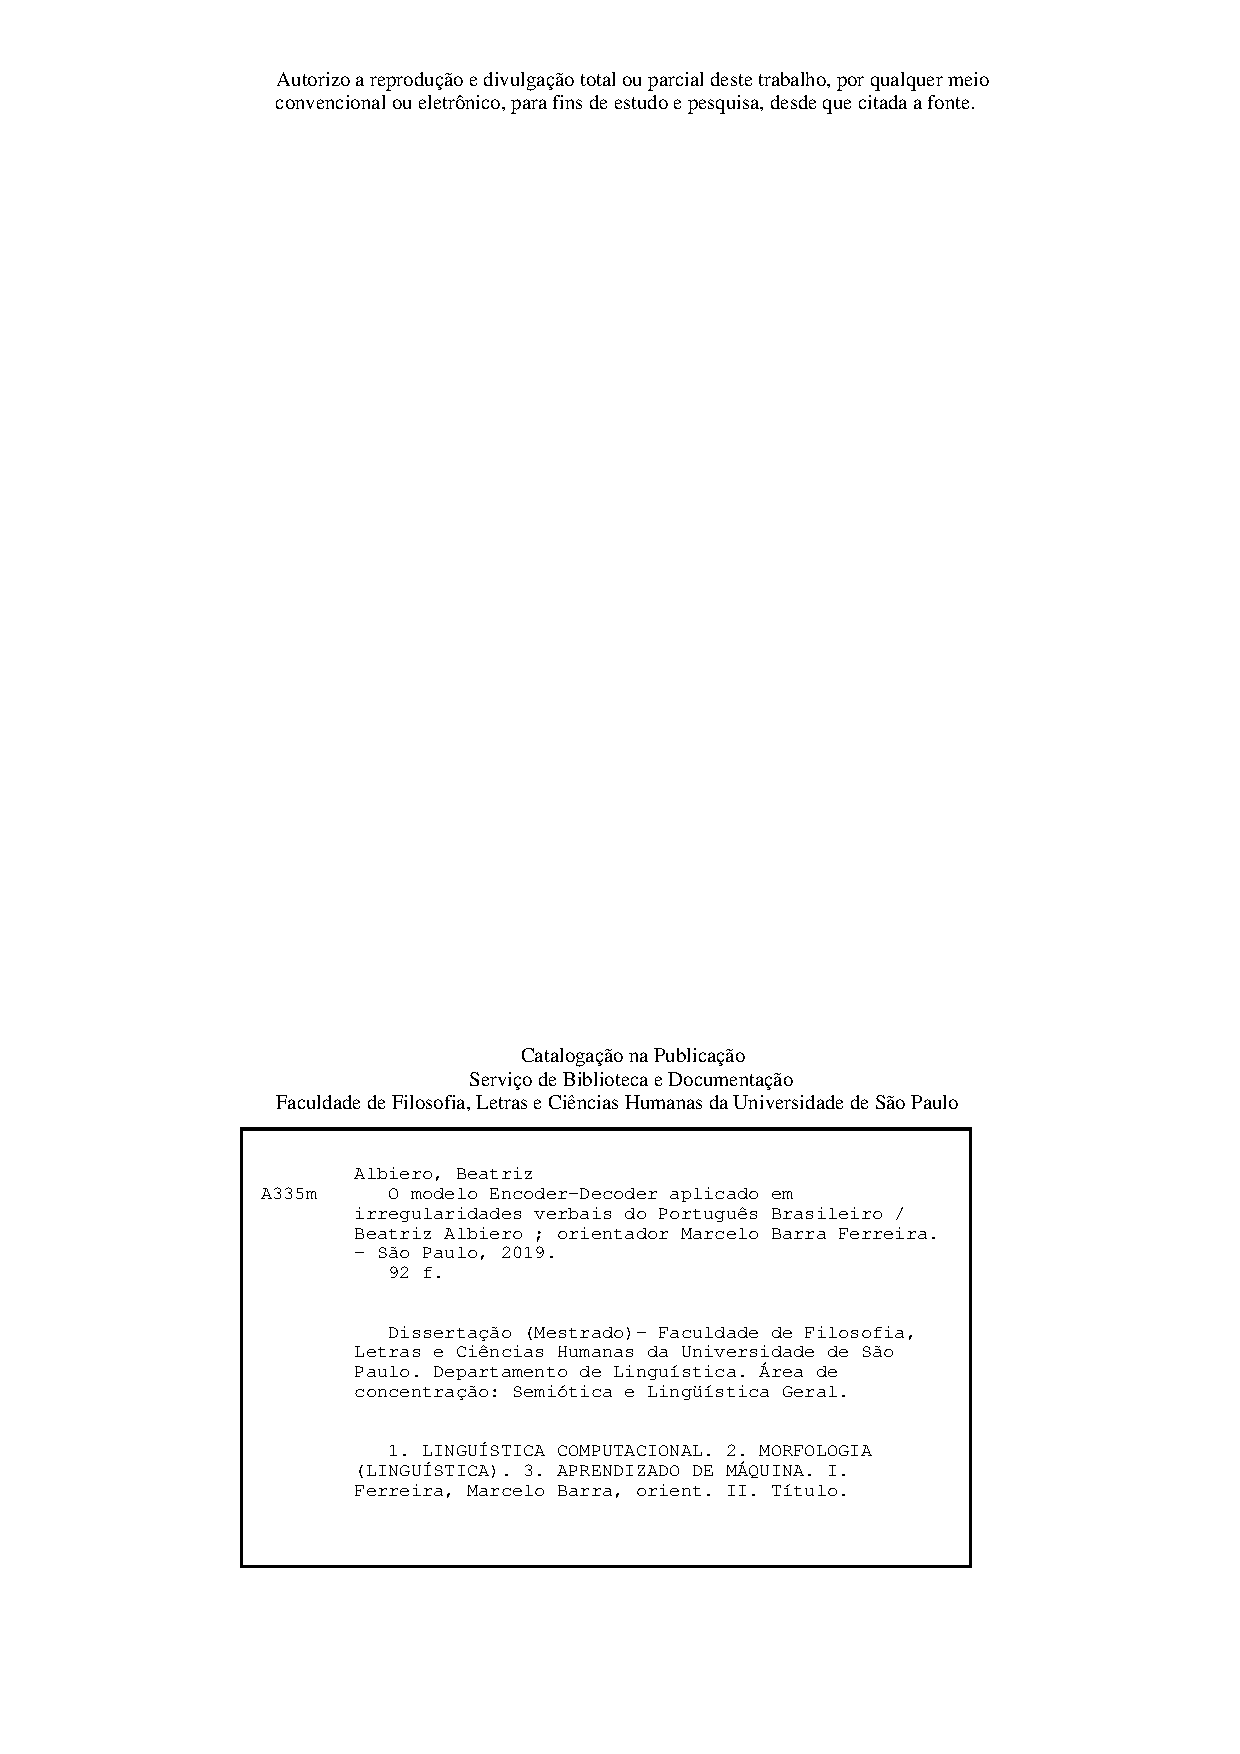
\includepdf[pagecommand={\thispagestyle{plain}},
%   pages=-]{fichacatalografica.pdf}
% %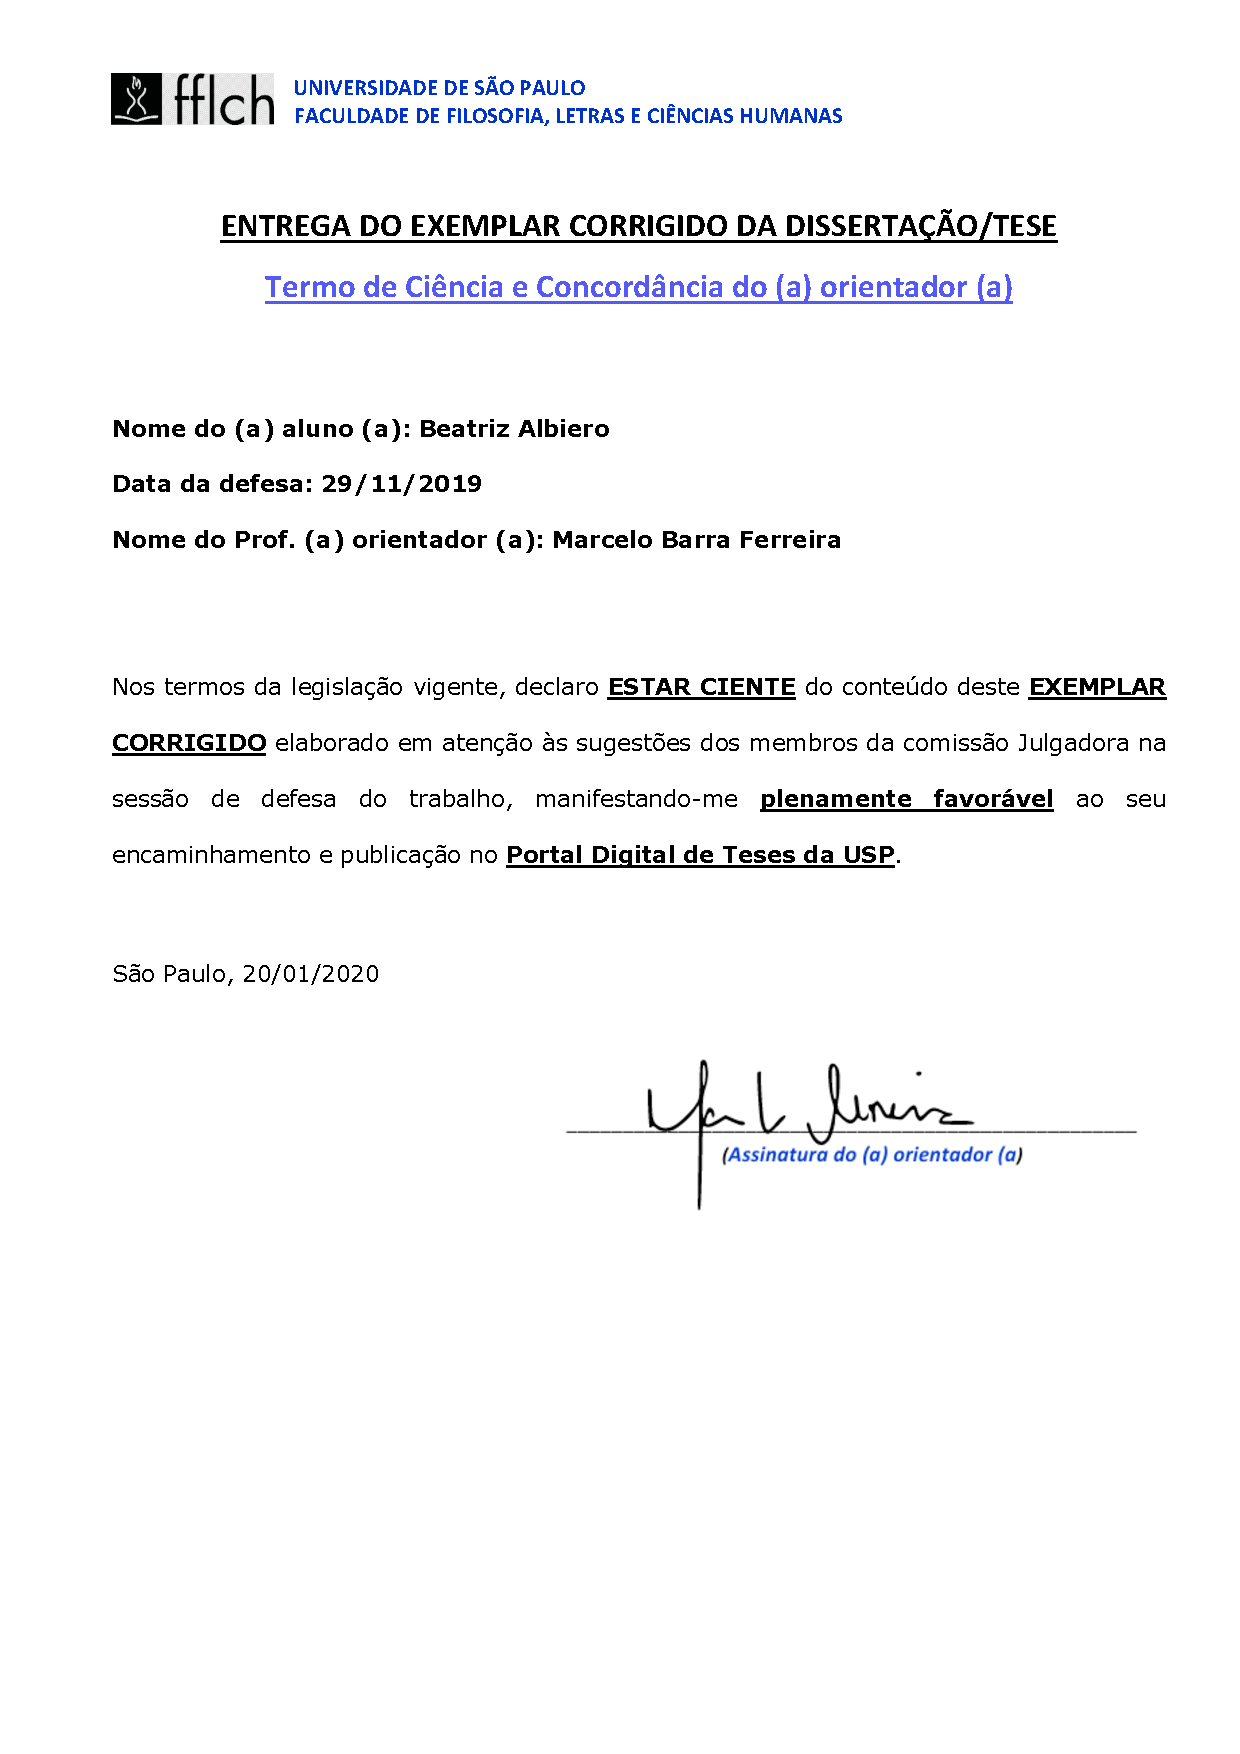
\includepdf[pagecommand={\thispagestyle{plain}},
%   pages=-]{termocienciaeditado.pdf}
%\chapter*{Banca Examinadora}
\thispagestyle{empty}

  %\textbf{\Large{Banca Examinadora}}
  \vskip 2cm
    \_\_\_\_\_\_\_\_\_\_\_\_\_\_\_\_\_\_\_
  
    Prof. Dr. Marcelo Barra Ferreira (USP)
    
    Presidente
    \vskip 2cm
    
    \_\_\_\_\_\_\_\_\_\_\_\_\_\_\_\_\_\_\_
    
    Profa. Dra. Livy Maria Real Coelho
    
    Membro titular
    \vskip 2cm
    
    \_\_\_\_\_\_\_\_\_\_\_\_\_\_\_\_\_\_\_
      
    Prof. Dr. Marcos Fernando Lopes (USP)

    Membro titular

    \vskip 2cm
    \_\_\_\_\_\_\_\_\_\_\_\_\_\_\_\_\_\_\_
    

    Prof. Dr. Pablo Picasso Feliciano de Faria (UNICAMP) 
    
    Membro titular
 
 

% ---------------------------------------------------------------------------- %
% Dedicatória
%\newenvironment{dedication}
  {%\clearpage           % we want a new page          %% I commented this
   \thispagestyle{empty}% no header and footer
   \vspace*{\stretch{10}}% some space at the top
   \itshape             % the text is in italics
   \raggedleft          % flush to the right margin
  }
  {\par % end the paragraph
   \vspace{\stretch{2}} % space at bottom is three times that at the top
   \clearpage           % finish off the page
  }

 \frontmatter              %% better to use this in book class
 \chapter{}
  \begin{dedication}
    Em memória de Valéria. 
    
    Mãe, amiga, querida. 
    \par   %% or a blank line
    \vspace{2\baselineskip}
    Ao meu pai André, que me deu a maior força 
    
    para começar, continuar e concluir este trabalho.
    
  \end{dedication}

% ---------------------------------------------------------------------------- %
% Agradecimentos

% %\chapter*{Agradecimentos}
% \pagenumbering{gobble}

% Posso dizer que eu tive ao meu lado pessoas muito importantes que me ajudaram a passar pela experiência do mestrado de forma incrível. Foram muitos desafios e aprendizados, e sem as pessoas listadas a seguir, certamente esse processo não teria sido tão produtivo. 

% Primeiramente, agradeço à minha família, que me apoiou e incentivou nos meus estudos desde sempre. À minha mãe Valéria, que apesar de não ter tido a oportunidade de acompanhar essa fase da minha vida, observa de longe e se faz presente a cada passo que dou. Não sinto saudades, pois sinto que está comigo sempre. Ao meu pai André, meus avós Astrid e Norberto e aos meus irmãos Fábio e Juliana, pelo amor, carinho e cuidado.

% Sou muito grata também ao meu orientador Marcelo Barra Ferreira. Tenho a sorte de poder dizer que a minha experiência no mestrado foi muito positiva e enriquecedora em um momento muito delicado para a pós-graduação brasileira, e certamente a sua orientação e parceria foi fundamental nesse processo.

% Agradeço aos meus amigos e membros do grupo de estudos em linguística computacional da USP (o GLIC), que me ajudaram e inspiraram. Agradecimentos especiais ao meu colega Bruno Guide, que me ajudou diversas vezes com as minhas questões sobre a pós, muito antes da minha pesquisa começar. Também agradeço à Livy pelo seu olhar crítico e curioso sempre. A forma como todos do grupo amam estudar linguística é incrível. Também agradeço ao querido professor Marcos Lopes, cuja participação também foi fundamental para a minha formação acadêmica e para que o meu ingresso no mundo da linguística ocorresse de maneira leve e agradável.

% Agradeço também aos meus colegas do Datalab, que me apoiaram e incentivaram durante a execução desta pesquisa. Sinto-me muito privilegiada por ter tido o apoio que eu tive no meu ambiente de trabalho e por todas as oportunidades que me foram concedidas para o meu desenvolvimento acadêmico. Agradecimento especial a Estêvão Uyrá, que contribuiu diretamente na execução desta pesquisa com sugestões valiosíssimas. Também sou muito grata ao professor Renato Vicente por ter me incluído em um time tão genial e criativo, além de todo o apoio na minha formação acadêmica e profissional. Também agradeço aos meus colegas Sami e Ricardo, pela compreensão, pelos conselhos e risadas.

% Também não posso deixar de agradecer ao meu colega Felipe Salvatore, doutorando no IME-USP, que me auxiliou com sugestões essenciais para a base computacional desta pesquisa. Às professoras Esmeralda Vailati Negrão e Maria Cristina Altman que me apresentaram ao universo da linguística e me incentivaram a estudar esse assunto com mais profundidade no mestrado.

% Finalmente, a todos aqueles que me apoiaram nos momentos mais difíceis, em especial: Maria Teresa Lamberte, Carlos Joventino, Arthur Athayde, Ramon Vilarino, Thaís Dresch, Marina Nagata e Manu Bonfim. 

% ---------------------------------------------------------------------------- %
% Abstract
% \chapter*{Resumo}
% \pagenumbering{gobble}
% \noindent Albiero, B. \textbf{O modelo Encoder-Decoder aplicado em irregularidades verbais do Português Brasileiro}. 
% 2019.
% Dissertação (Mestrado) - Faculdade de Filosofia e Ciências Humanas,
% Universidade de São Paulo, São Paulo, 2019.
% \\

% Inspirada na controversa questão da aquisição de verbos irregulares na língua inglesa (\cite{chomsky:1968},  \cite{Pinker:1988},
% \cite{Albright2003RulesVA}, \cite{kirov:2018}), esta pesquisa tem como objetivo estudar a questão da flexão de verbos irregulares do Português Brasileiro sob a ótica do modelo computacional \textit{Encoder-Decoder}. Para tanto, a tarefa proposta ao modelo era a de predizer uma forma verbal flexionada dada uma forma primária (\textit{Radical + Vogal Temática}). O escopo da pesquisa restringiu-se ao estudo do paradigma de 1\aup{a} Pessoa do Singular no Modo Indicativo e Tempo Presente. O modelo utilizado, por sua vez, é um modelo de caráter associativo que pertence ao grupo dos modelos de Redes Neurais Artificiais. Também, fez-se necessária a construção de um \textit{corpus} linguístico composto pelo paradigma selecionado e em seguida transcrito em notação fonética específica para viabilizar a utilização do modelo escolhido. O \textit{corpus} produzido é composto por 423 verbos que foram marcados como pertencendo às famílias de verbos regulares (51\%) ou irregulares (49\%). Ainda, dentro do escopo da família de verbos irregulares, foi possível identificar 15 subgrupos conforme a identificação de diferentes padrões de flexão. A partir da notação fonética utilizada, os verbos puderam ser associados a novas representações que englobavam informações relativas aos traços fonéticos presentes. Assim, o modelo proposto tenta predizer as formas flexionadas a partir da identificação das relações fonéticas envolvidas durante o processo de flexão. O modelo apresentado foi submetido a múltiplos treinamentos e testes e apresentou uma acurácia média de 13.55\%, mas chegou a acertar 17\% em um dos experimentos. Considerando a segmentação entre verbos regulares e irregulares, o modelo performou melhor na classe dos regulares. Entretanto, considerando-se todas as 16 classes individualmente (15 irregulares + 1 regular), pôde-se observar que as duas primeiras classes em que o modelo performou melhor eram classes irregulares, deixando a classe regular como a terceira com os melhores resultados.

% \\
%  \textbf{Palavras-chave:}
% morfologia verbal, aprendizagem de máquina, conexionismo.

\chapter*{Abstract}
\pagenumbering{gobble}
\noindent Albiero, B. \textbf{The Encoder-Decoder Model Applied to Brazilian-Portuguese Verbal Irregularities}. 
2019.
Dissertação (Mestrado) - Faculdade de Filosofia e Ciências Humanas,
Universidade de São Paulo, São Paulo, 2019.
\\

Inspired by the controversial debate about the acquisition of irregular verbs in English language (\cite{chomsky:1968}, \cite{Pinker:1988},
\cite{Albright2003RulesVA}, \cite{kirov:2018}), this research aims to study the inflection process of irregular verbs in Portuguese through the perspective of the computational model \textit{Encoder-Decoder}. To do this, we proposed the task of predicting an inflected verbal form given a primary form (\textit{Stem + Thematic Vowel}). The scope of the research was restricted to the study of the singular first-person paradigm in the indicative mood and present tense. The model, in turn, is an associative model that belongs to the group of Artificial Neural Networks models. Also, it was necessary to construct a linguistic \textit{corpus} composed by the chosen paradigm and then transcribe it into a specific phonetic notation to enable the usage of the chosen model. The resulting \textit{corpus} consists of 423 verbs that were marked as belonging to either regular (51\%) or irregular (49\%) verb families. Moreover, within the scope of irregular verbs, it was possible to identify 15 subgroups through the identification of inflection patterns. Through the phonetic notation provided, verbs could be associated with new representations that included information related to the phonetic features. Thus, the proposed model attempts to predict inflected forms by identifying the involved phonetic relationships during the inflection process. The model was submitted to multiple trainings and tests and presented an average accuracy of 13.55\%, but it got to 17\% in one of the experiments. Considering the segmentation between regular and irregular verbs, the model performed better among the regular class. However, considering all 16 classes individually (15 irregular + 1 regular), it was observed that the first two classes in which the model performed best were irregular classes, leaving the regular class with the third place.

\textbf{Key-words:}
verbal morphology, machine learning, connectionism.

% \tableofcontents
\pagestyle{fancy}
\onehalfspacing            % espaçamento um e meio
\mainmatter
\pagenumbering{arabic}
\chapter*{Introduction}
\addcontentsline{toc}{chapter}{Introdução}

% Inspirada no controverso tema da aquisição de verbos irregulares na língua inglesa
% (\cite{Pinker:1999}, \cite{chomsky:1968},  \cite{Pinker:1988}, \cite{rumelhart:1986}), esta pesquisa tem como objetivo estudar o processo de flexão de verbos irregulares do Português Brasileiro fazendo uso de um modelo computacional conhecido como \textit{Encoder-Decoder} (\cite{enc-dec:2014}).

% A controvérsia em torno do processo de aprendizado de verbos irregulares teve início na década de 60, tendo sido explorada por pesquisadores de diversas áreas (linguistas, psicólogos, neurocientistas, cientistas da computação, entre outros). No Cap. \ref{ch:01} deste trabalho, serão apresentadas as origens e motivações da discussão, bem como os principais pesquisadores envolvidos e hipóteses levantadas. Além disso, será introduzida uma categoria de modelos computacionais associativos conhecida como Rede Neural Artificial, do qual o modelo \textit{Encoder-Decoder} faz parte. Em seguida, na primeira parte da seção de motivação (Seç. \ref{sec:motivation}) serão apontadas algumas especificidades gramaticais da língua portuguesa que podem dificultar o processo de aprendizado da flexão irregular. Na segunda parte da seção, serão apresentados alguns trabalhos computacionais que se seguiram nos anos subsequentes em resposta à discussão estabelecida. 

Inspired by the great controversy regarding the acquisition of irregular verbs in the English language
(\cite{Pinker:1999}, \cite{chomsky:1968}, \cite{Pinker:1988}, \cite{rumelhart:1986}), this research aims to study the inflection process of Brazilian Portuguese irregular verbs making use of a computational model known as \textit{Encoder-Decoder} (\cite{enc-dec:2014}).

The debate surrounding the process of learning irregular verbs started in the 1960s, having been explored by researchers from different fields (linguists, psychologists, neuroscientists, computer scientists, among others). In Chap. \Ref{ch:01}, we present the origins and motivations of the discussion, as well as the main researchers involved and raised hypotheses. In addition, a category of associative computational models known as the Artificial Neural Network will be introduced, of which the \textit{Encoder-Decoder} model is part. Next, in the first part of the motivation section (Sec. \Ref{sec:motivation}) we point out some grammatical specificities of the Portuguese language that could hinder the learning process of irregular inflection. In the second part of the section, we will present a historical review regarding the computational contributions that followed in response to the discussion.

% Após a exposição dos diferentes trabalhos desenvolvidos, ficará evidente a razão pela qual tal tema chamou a atenção de tantas áreas distintas. Ademais, veremos que o problema da flexão de verbos irregulares tornou-se um desafio computacional para além dos problemas linguísticos ou cognitivos em questão, de modo que muitas pesquisas subsequentes acabaram se distanciando do debate linguístico e focando nos aspectos matemáticos que viabilizariam o aprendizado artificial. A presente pesquisa também dará continuidade a esse aspecto computacional do problema e não terá como objetivo assumir qualquer posição em torno dos aspectos cognitivos do debate. Desse modo, avaliaremos o uso do modelo \textit{Encoder-Decoder} a partir de um ponto de vista prático de acordo com a sua performance na tarefa proposta e em comparação a outros modelos computacionais já apresentados em outras pesquisas.

After the exhibition of the different conducted studies, it will become evident why this theme caught the attention of so many different areas. Moreover, we will see that the problem of inflecting irregular verbs has become a computational challenge beyond the linguistic or cognitive issues under debate, in such a way that many subsequent researches have ended up distancing themselves from the linguistic matters and focused on the mathematical aspects that would make artificial learning feasible. This research will also continue this computational aspect of the problem and will not aim to take any side regarding the cognitive aspects of the debate. In this way, we will evaluate the use of the \textit{Encoder-Decoder} model from a practical point of view according to its performance in the proposed task and in comparison to other computational models already presented in other research.

To achieve the proposed objective, the first stage of this research was the development of a specific linguistic corpus for the task. The resulting corpus is presented in full in the Appendix (B), but will be discussed in detail in Chap. 2, in Sec. \ref{sec:corpus}. Still in this chapter, we will see the importance of applying appropriate preprocessing treatments in the units of the corpus to enable the intended learning. For that, we will revisit a preprocessing algorithm proposed in a previous work, carried out by \cite{rumelhart:1986}. Then, we will present the preprocessing algorithm developed in this research.

Chapter 3 introduces basic concepts regarding the subject of \textit{Machine Learning} and then present an introduction to Artificial Neural Network models. In addition, we will address the concepts of \textit{Language Models} and architectures of \textit{Recurring Neural Networks} - essential issues for understanding the highlighted model of this research, the \textit{Encoder-Decoder}. After making the necessary introductions, we will be ready to present the \textit{Encoder-Decoder} model in Chapter 4.  

Chapter 5, in turn, will present and discuss the results obtained. In it we will see the settings chosen for the definition of the model and the metrics used for its evaluation. We will also analyze the different errors observed and look for possible explanations for the results obtained.

To conclude, Chapter 6 will display a summary of the subjects covered in this research and also point out suggestions for future research on the subject.





\fancyhead[RE,LO]{\thesection}
\chapter{Learning Irregular Verbs}
\label{ch:01}

The first part of this chapter will be dedicated to a presentation regarding the origin of the discussion about the inflectional learning process of irregular verbs. Thus, we will build an overview of the problem and present the main hypotheses and research involved. Then, we will discuss the motivations that led to the production of this research. In this sense, we will see that, on the one hand, there is a linguistic interest, motivated by a greater complexity of the Portuguese language compared to English. On the other hand, we will also see that there is a computational interest, motivated by the emergence of new modeling resources. Finally, we will see a section aimed at delimiting the scope of the research.

\section{Context}
In the field of Language Acquisition, the problem regarding the inflection process of irregular verbs in the English language is certainly among one of the most controversial topics of debate in Linguistics (\cite{chomsky:1968}, \cite{Pinker:1999}, \cite{Pinker:1988}, \cite{Albright2003RulesVA}, \cite{kirov:2018}). The heart of the debate is the exact characterization of the mechanisms that enable a speaker to be able to relate a verb in its non-inflected form (\textit{walk}, for example) to its inflected form in \textit{Simple Past} (\textit{walked}).

Past tense verbs in English can be subdivided into a variety of families. A first group would be the set of \textit{regular verbs}, whose form corresponds to the application of the rule \textit{\text{root} + ed} (as in the example seen from the verb \textit{to walk}).
Among the irregular verbs, these can be considered suppletive, that is, they have a unique inflection process and no apparent rule, such as \textit{go} $ \rightarrow $ \textit{went}, or they can conglomerate following phonetic patterns (\cite{Nelson:2010}):

\begin{enumerate}
    \item blow – blew, grow – grew, know – knew, throw – threw
    \item bear – bore, swear – swore, tear – tore, wear – wore
    \item drink – drank, shrink – shrank, sink – sank, stink – stank 
\end{enumerate}

One could think that the learning of such patterns would depend on a case by case memorization. However, \cite{Bybee:1983} shows a psycholinguistic study in which individuals are presented with several invented verbs (hypothetically in a non-inflected form). The research revealed that, instead of systematically applying the regular rule (verb + \textit{ed}), individuals showed tendencies to allocate some verbs in some irregular subgroups. For example, for the invented verb “\textit{spling}”, most individuals chose the form “\textit{splang}” or “\textit{splung}”. This example contradicts the idea that speakers could be simply reproducing memorized forms and suggests that they are actively identifying patterns. In addition, they have a natural intuition about the appropriateness of allocating a verb to one group of verbs or another.

From the given example, it is reasonable to think that the motivation behind such trends occurs from the similarities between the phonetic units of the invented verbs and the real verbs that already have an irregular character inflection. However, the circumstances that lead to the acquisition of this linguistic \textit{intuition} are undetermined. On the one hand, it makes sense to say that for a human being to be able to be introduced into the world of speakers, it would require some inherited capabilities, otherwise the learning process would not be possible. In contrast, studies show that children deprived of contact with a speaking society are permanently unable to fully master the grammar of a language (\cite{Pinker:languageinstinct}), which leads us to conclude that children's experience with society, as well as their own genetic pre-dispositions are both partly responsible for the language development process. The difficulty, therefore, is in the attempt to quantify, delimit and point out the knowledge acquired from cultural contact, as well as the so-called \textit{inate} linguistic knowledge. It is, therefore, around this issue that the debate about the learning of irregular verbs in the English language begins.

On one side of the debate, there is the theory of Generative Phonology by Chomsky and Halle (\citeyear{chomsky:1968}). In this theory, individuals would be carriers of a language acquisition device (\textit{LAD} ) responsible for \textit{formulating} and \textit{manipulating} abstract phonological structures in a system of rules. In a simplified way, the theory proposes that the speaker is able to intuitively identify and formulate rules to account for the learning of irregular forms of the language. An example of this is the family of verbs ending in "-ind".

\begin{center}
bind – bound, find – found, grind – ground, wind – wound
\end{center}

We can see that, in a simplified way, a rule can be proposed as:

\begin{center}
a\textsci $\rightarrow$ a\textupsilon / \textbf{X}  \_\_nd]+past
\end{center}

The proposed rule suggests that the segment [a \textsci] becomes [a \textupsilon] when followed by [nd] and inflected to the past. The symbol \_ \_ represents the place where such a transformation occurs and \textbf{X} represents an arbitrary phonological unit.

In other words, it can be said that the knowledge said \textit{innate} defended by Chomsky and Halle refers to a certain cognitive capacity for formulating rules from the identification of some fundamental elements (such as the elements pointed out in the proposed rule). Such a structure would allow speakers to build generalizations and, eventually, abstract the phonological rules of their language. \\

On the other side of the debate, the researchers \cite{rumelhart:1986} confront the previous theory by arguing that behaviors of a regulated character can be reproduced by mechanisms that do not depend on any symbolic manipulation. Instead, the researchers suggest that the mechanisms involved in the verbal inflection process can be constructed in such a way that its performance can be described through rules, but that the rules themselves are not explicitly represented in any part of the process. To support this idea, \cite{rumelhart:1986} present a computational model based on associative patterns that do not use constructions with rules of this type. Subsequently, the model built was fundamental for the emergence of a new school within the cognitive sciences: connectionism. \\

\definecolor{blue}{RGB}{159, 192, 176}
\definecolor{green}{RGB}{160, 227, 127}
\definecolor{orange}{RGB}{243, 188, 125}
\definecolor{red}{RGB}{253, 123, 84}
\definecolor{nephritis}{RGB}{39, 174, 96}
\definecolor{emerald}{RGB}{46, 204, 113}
\definecolor{turquoise}{RGB}{39, 174, 96}
\definecolor{green-sea}{RGB}{22, 160, 133}
\definecolor{purple}{RGB}{181, 124, 215}
% Tikzstyles for Computation Graphs

% nodes
\tikzstyle{noop} = [circle, draw=none, fill=red, minimum size = 10pt]
\tikzstyle{op} = [circle, draw=red, line width=1.5pt, fill=red!70, text=black, text centered, font=\bf \normalsize, minimum size = 25pt]

\tikzstyle{opintense} = [circle, draw=red, line width=1.5pt, fill=red!150, text=black, text centered, font=\bf \normalsize, minimum size = 25pt]


%new style
\tikzstyle{gp} = [circle, draw=red, line width=4pt, text=black, text centered, font=\bf \normalsize, minimum size = 4.cm]

\tikzstyle{box} = [rectangle, draw=red, line width=1.5pt, fill=red!70, text=black, align=center, font=\bf \normalsize, minimum size = 45pt]

\tikzstyle{box2} = [rectangle, draw=black, line width=0.9pt, text=black, align=center, font=\bf \normalsize, minimum size = 20pt]

\tikzstyle{box3} = [rectangle, draw=black, line width=0.9pt, fill=black, text=white, align=center, font=\bf \normalsize, minimum size = 20pt]

\tikzstyle{box4} = [rectangle, draw=black, line width=0.9pt, text=black, align=center, font=\bf \normalsize, minimum size = 20pt]

\tikzstyle{state} = [circle, draw=blue, line width=1.5pt, fill=blue!70, text=black, text centered, font=\bf \normalsize, minimum size = 25pt]

\tikzstyle{output} = [circle, draw=purple, line width=1.5pt, fill=purple!70, text=black, text centered, font=\bf \normalsize, minimum size = 25pt]


\tikzstyle{gradient} = [circle, draw=nephritis, line width=1.5pt, fill=nephritis!60, text=black, text centered, font=\bf \normalsize, minimum size = 25pt]
\tikzstyle{textonly} = [draw=none, fill=none, text centered, font=\bf \normalsize]
\tikzstyle{boxtextonly} = [draw=none, fill=none, align=center, font=\bf \normalsize]

\tikzstyle{normal} = [circle, draw=black, line width=1.0pt, fill=none, text=black, text centered, font=\bf \normalsize, minimum size = 20pt]

\tikzstyle{normal_dashed} = [circle, draw=black, line width=1.0pt, dashed, fill=none, text=black, text centered, font=\bf \normalsize, minimum size = 10pt]


% edges
\tikzstyle{tedge}  = [draw, thick, >=latex, ->]
\tikzstyle{tedge_dashed}  = [draw, thick, >=latex, ->, dashed]
\tikzstyle{nedge}  = [draw, thick, >=latex]
\tikzstyle{nedge_dashed}  = [draw, thick, >=latex, dashed]

\tikzstyle{arrows_dashed}  = [draw, thick, >=latex, <->, dashed]

\tikzstyle{tedge_test} = [draw,->,out=45,in=225]


% namedscope
\tikzstyle{namedscope} = [circle, draw=orange, line width=1.5pt, fill=orange!60, align=center, inner sep=0pt]

%round
\tikzset{
    %Define standard arrow tip
    >=stealth',
        punkt/.style={
           rectangle,
           rounded corners,
           draw=black, very thick,
           text width=6.5em,
           minimum height=2em,
           text centered},
    % Define arrow style
    pil/.style={
           ->,
           thick,
           draw=red,
           shorten <=10pt,
           shorten >=10pt,}
}

\begin{figure}[ht!]
\centering

\scalebox{1.0}{
\begin{tikzpicture}[auto]

% operations =========
% phon features 1
\node[textonly] (1pho1) {plosive-vogal-plosive};

% Legenda
\node[textonly, above=10pt of 1pho1] (leg1) {Input Units};


% FNN input
\node[normal, right=5pt of 1pho1] (x1) {};
\node[normal, below=25pt of x1] (x2) {};
\node[normal, below=25pt of x2] (x3) {};
\node[normal, below=25pt of x3] (x4) {};
\node[normal, below=25pt of x4] (x5) {};
\node[normal, below=25pt of x5] (x6) {};
\node[text, below=10pt of x6] (nada) {};

% FNN output
\node[normal, right=45pt of x1] (y1) {};
\node[normal, right=45pt of x2] (y2) {};
\node[normal, right=45pt of x3] (y3) {};
\node[normal, right=45pt of x4] (y4) {};
\node[normal, right=45pt of x5] (y5) {};
\node[normal, right=45pt of x6] (y6) {};

% phon features 2
\node[textonly, right=5pt of y1] (2pho1) {plosive-vowel-plosive};
\node[textonly, above=10pt of 2pho1] (leg2) {Output Units};
\node[textonly, left=25pt of x2] (1pho2) {front-nasal-back};
\node[textonly, right=25pt of y2] (2pho2) {front-nasal-back};
\node[textonly, left=25pt of x3] (3pho1) {...};
\node[textonly, right=25pt of y3] (1pho3) {...};
\node[textonly, left=25pt of x4] (4pho1) {nasal-cont-plosive};
\node[textonly, right=25pt of y4] (1pho4) {nasal-cont-plosive};
\node[textonly, left=25pt of x5] (5pho1) {middle-fric-low};
\node[textonly, right=25pt of y5] (1pho5) {middle-fric-low};
\node[textonly, left=25pt of x6] (6pho1) {vowel-fricative-\#};
\node[textonly, right=25pt of y6] (1pho6) {vowel-fric-\#};
% edges FNN
\path[nedge] (x1) -- (y1);
\path[nedge] (x1) -- (y2);
\path[nedge] (x1) -- (y3);
\path[nedge] (x1) -- (y4);
\path[nedge] (x1) -- (y5);
\path[nedge] (x1) -- (y6);
\path[nedge] (x2) -- (y1);
\path[nedge] (x2) -- (y2);
\path[nedge] (x2) -- (y3);
\path[nedge] (x2) -- (y4);
\path[nedge] (x2) -- (y5);
\path[nedge] (x2) -- (y6);
\path[nedge] (x3) -- (y1);
\path[nedge] (x3) -- (y2);
\path[nedge] (x3) -- (y3);
\path[nedge] (x3) -- (y4);
\path[nedge] (x3) -- (y5);
\path[nedge] (x3) -- (y6);
\path[nedge] (x4) -- (y1);
\path[nedge] (x4) -- (y2);
\path[nedge] (x4) -- (y3);
\path[nedge] (x4) -- (y4);
\path[nedge] (x4) -- (y5);
\path[nedge] (x4) -- (y6);
\path[nedge] (x5) -- (y1);
\path[nedge] (x5) -- (y2);
\path[nedge] (x5) -- (y3);
\path[nedge] (x5) -- (y4);
\path[nedge] (x5) -- (y5);
\path[nedge] (x5) -- (y6);
\path[nedge] (x6) -- (y1);
\path[nedge] (x6) -- (y2);
\path[nedge] (x6) -- (y3);
\path[nedge] (x6) -- (y4);
\path[nedge] (x6) -- (y5);
\path[nedge] (x6) -- (y6);


\end{tikzpicture}
}\caption{Model Scheme proposed by researchers Rumelhart and McClelland} 
\label{fig:esquemafdd}
\end{figure}


The model was created by analogy to the structure in which neurons in the brain relate. It is basically composed of an artificial network of nodes interconnected in parallel (Fig. \ref{fig:esquemafdd}).

The first layer of nodes in the model is responsible for receiving the input data, which are the data regarding the distinctive phonetic features that characterize the sounds of a verb in its root form. Phonetic features can be characterized as distinctive properties of phonic units (\cite{paraconhecer:2015}). Such properties can be based on acoustic, articulatory or perceptual criteria. In the figure, each node is shown next to a sequence of three features. The first node, for example, refers to the sequence \textbf{plosive-vowel-plosive}. In this case, \textit{plosive} indicates a common property among some consonants, related to the interruption of the air flow (as in the phone [k], for example). In the figure we still have \textbf{fric} for fricatives, \textbf{vowel} for vowels, \textbf{nasal} for nasality, places of execution (\textbf{front} and \textbf{back}), tongue features (\textbf{middle}, \textbf {low}), among others. Still on the \textit{input} layer, it is possible to observe that each node is represented by a triad of phonetic features. This was the solution provided by the authors to perform the mapping between the features of the verbs in their root form to their \textit{Past Simple}. The \textit{inputs} are structured in this way to overcome the difficulty of inserting data of a sequential nature and of variable size (as is the case of a verb - composed of a sequence of sounds). Each triad is an association of three features, each referring to a phone. For example, for the verb \textit{came} (transcribed in phonetic form by the authors as \textit{/kAm/}), each phone has multiple features. The phone [\textit{k}], for example, is an plosive, voiceless and "back" consonant. Subsequent phones are also composed by their respective phonetic features, in such a way that we can represent the verb as a sequence of lists of phonetic features (Table \ref{tab:trigrams}). The topic regarding the phonetic features used in this research, as well as the entire preprocessing scheme used by the authors \cite{rumelhart:1986} will be discussed in greater depth in Chap. \ref{ch:02}.

\begin{table}[H]
\begin{center}
\begin{tabular}{ccc}
k                    & A                    & m                    \\ \hline
voiceless                & long                & nasal                \\
interrupted         & vowel               & interrupted         \\
back            & low                & front            \\
consonant           & front            & consonant            \\
\multicolumn{1}{l}{} & \multicolumn{1}{l}{} & \multicolumn{1}{l}{}
\end{tabular}
\caption{Trigrams of Phonetic Features Used as  \textit{Inputs} to Rumelhart and McClelland's model}
\label{tab:trigrams}
\end{center}
\end{table}

Returning to Fig.\ref{fig:esquemafdd}, we see a network of connections after the \textit{input} layer. Each connection, in turn, has a \textit{weight}. These weights will act as a kind of \textit{input} filter, making weights with higher values pass the information on with more effect (or strength), and smaller weights with less. The second layer of nodules in Fig. \ref{fig:esquemafdd} is a response layer (known as a \textit{output} layer) that aims to return data regarding the features that characterize the sounds of the same verb provided in \textit{input}, but in \textit{Simple Past}.

During the learning process of the model, the output data from the \textit{output} layer must then be compared to the correct form of the verb in the past tense, through a kind of template, known as \textit{target} (Fig. \ref{fig:gabarito}). Having made this comparison, it is possible to change the network of connections between \textit{input} and \textit{output} layers in order to reinforce (or weaken) their weights to achieve the proposed learning. Before the first comparison, the network is initialized with random weights. As the number of comparisons increases, the tendency is for the weights to be gradually calibrated in order for the model to reach its objective, which in this case, is to learn the inflection patterns of the verbs.

\definecolor{blue}{RGB}{159, 192, 176}
\definecolor{green}{RGB}{160, 227, 127}
\definecolor{orange}{RGB}{243, 188, 125}
\definecolor{red}{RGB}{253, 123, 84}
\definecolor{nephritis}{RGB}{39, 174, 96}
\definecolor{emerald}{RGB}{46, 204, 113}
\definecolor{turquoise}{RGB}{39, 174, 96}
\definecolor{green-sea}{RGB}{22, 160, 133}
\definecolor{purple}{RGB}{181, 124, 215}
% Tikzstyles for Computation Graphs

% nodes
\tikzstyle{noop} = [circle, draw=none, fill=red, minimum size = 10pt]
\tikzstyle{op} = [circle, draw=red, line width=1.5pt, fill=red!70, text=black, text centered, font=\bf \normalsize, minimum size = 25pt]

\tikzstyle{opintense} = [circle, draw=red, line width=1.5pt, fill=red!150, text=black, text centered, font=\bf \normalsize, minimum size = 25pt]


%new style
\tikzstyle{gp} = [circle, draw=red, line width=4pt, text=black, text centered, font=\bf \normalsize, minimum size = 4.cm]

\tikzstyle{box} = [rectangle, draw=red, line width=1.5pt, fill=red!70, text=black, align=center, font=\bf \normalsize, minimum size = 45pt]

\tikzstyle{box2} = [rectangle, draw=black, line width=0.9pt, text=black, align=center, font=\bf \normalsize, minimum size = 20pt]

\tikzstyle{box3} = [rectangle, draw=black, line width=0.9pt, fill=black, text=white, align=center, font=\bf \normalsize, minimum size = 20pt]

\tikzstyle{box4} = [rectangle, draw=black, line width=0.9pt, text=black, align=center, font=\bf \normalsize, minimum size = 20pt]

\tikzstyle{state} = [circle, draw=blue, line width=1.5pt, fill=blue!70, text=black, text centered, font=\bf \normalsize, minimum size = 25pt]

\tikzstyle{output} = [circle, draw=purple, line width=1.5pt, fill=purple!70, text=black, text centered, font=\bf \normalsize, minimum size = 25pt]


\tikzstyle{gradient} = [circle, draw=nephritis, line width=1.5pt, fill=nephritis!60, text=black, text centered, font=\bf \normalsize, minimum size = 25pt]
\tikzstyle{textonly} = [draw=none, fill=none, text centered, font=\bf \normalsize]
\tikzstyle{boxtextonly} = [draw=none, fill=none, align=center, font=\bf \normalsize]

\tikzstyle{normal} = [circle, draw=black, line width=1.0pt, fill=none, text=black, text centered, font=\bf \normalsize, minimum size = 20pt]

\tikzstyle{normal_dashed} = [circle, draw=black, line width=1.0pt, dashed, fill=none, text=black, text centered, font=\bf \normalsize, minimum size = 10pt]


% edges
\tikzstyle{tedge}  = [draw, thick, >=latex, ->]
\tikzstyle{tedge_dashed}  = [draw, thick, >=latex, ->, dashed]
\tikzstyle{nedge}  = [draw, thick, >=latex]
\tikzstyle{nedge_dashed}  = [draw, thick, >=latex, dashed]

\tikzstyle{arrows_dashed}  = [draw, thick, >=latex, <->, dashed]

\tikzstyle{tedge_test} = [draw,->,out=45,in=225]


% namedscope
\tikzstyle{namedscope} = [circle, draw=orange, line width=1.5pt, fill=orange!60, align=center, inner sep=0pt]

%round
\tikzset{
    %Define standard arrow tip
    >=stealth',
        punkt/.style={
           rectangle,
           rounded corners,
           draw=black, very thick,
           text width=6.5em,
           minimum height=2em,
           text centered},
    % Define arrow style
    pil/.style={
           ->,
           thick,
           draw=red,
           shorten <=10pt,
           shorten >=10pt,}
}

\begin{figure}[H]
\centering

\scalebox{1.0}{
\begin{tikzpicture}[auto]

% operations =========
% phon features 1
\node[textonly] (out1) {Output};
\node[textonly, right=50pt of out1] (gab) {Target};


% FNN output
\node[normal, below=40pt of out1] (x1) {$\hat{y_{1}}$};
\node[normal, below=35pt of x1] (x2) {$\hat{y_{2}}$};
\node[normal, below=35pt of x2] (x3) {$\hat{y_{3}}$};

% from input
\node[text, left=45pt of x1] (in1) {};
\node[text, left=45pt of x2] (in2) {};
\node[text, left=45pt of x3] (in3) {};


% comparison
\node[text, right=31pt of x1] (nada1) {};
\node[text, below=5pt of nada1] (nada2) {\small{Comparison}};
\node[text, below=10pt of out1] (update) {\small{Update}};
\node[text, right=31pt of x2] (nada6) {};
\node[text, right=31pt of x3] (nada7) {};

\node[text, left=31pt of x1] (nada3) {};
\node[text, left=31pt of x2] (nada4) {};
\node[text, left=31pt of x3] (nada5) {};


% FNN target
\node[normal, right=65pt of x1] (y1) {$y_{1}$};
\node[normal, right=65pt of x2] (y2) {$y_{2}$};
\node[normal, right=65pt of x3] (y3) {$y_{2}$};
\node[text, below=15pt of x3] (nada) {};



% edges FNN
\path[arrows_dashed] (x1) -- (y1);
\path[arrows_dashed] (x2) -- (y2);
\path[arrows_dashed] (x3) -- (y3);

\draw[arrows_dashed, ->] (nada1) to [out=135,in=115] (nada3);
\draw[arrows_dashed, ->] (nada6) to [out=135,in=115] (nada4);
\draw[arrows_dashed, ->] (nada7) to [out=135,in=115] (nada5);

\path[tedge] (in1) -- (x1);
\path[tedge] (in2) -- (x1);
\path[tedge] (in3) -- (x1);

\path[tedge] (in1) -- (x2);
\path[tedge] (in2) -- (x2);
\path[tedge] (in3) -- (x2);

\path[tedge] (in1) -- (x3);
\path[tedge] (in2) -- (x3);
\path[tedge] (in3) -- (x3);



\end{tikzpicture}
}\caption{Comparison between \textit{Output} and \textit{Target}} 
\label{fig:gabarito}
\end{figure}

To conduct the training, \cite{rumelhart:1986} fed 420 verbs into the model repeatedly (200 times each, 84,000 insertions in total). After training, the model was able to correctly reconstruct all of their irregular forms. In addition, in a new group with 86 unknown verbs, it hit about 2/3 of the set. Among the new irregular verbs, it made some interesting errors of \textit{overregularization} (such as \textit{catched} (instead of \textit{caught}) and  \textit{digged} (instead of \textit{dug})). These errors were observed in 11 of the 14 irregular verbs tested (\cite{pinker:1993}).

In addition to these results, \cite{rumelhart:1986} report that the model's learning process presents an interesting phenomenon, with a performance similar to behaviors observed in children during an acquisition phase: the U-Shaped Development Curve, \cite{marcus:1992}). The U-Shaped Development curve basically refers to a learning process that takes place in three stages: \\

(i) first, children can correctly reproduce the expected irregular inflection of verbs  (\textit{come}$\rightarrow$\textit{came});

(ii) next, they go through a process of \textit{overgeneralization} (in which they produce shapes like \textit{comed}) ;

(iii) finally, they start to correctly reproduce both regular and irregular verbs. \\


\cite{rumelhart:1986} describe how it was possible to observe such behavior in their model.
In the initial phase of the training process, the model was fed with a small amount of verbs, such as: \textit{come}, \textit{get}, \textit{give}, \textit {look}, \textit{take} , \textit{go}, \textit {have}, \textit {live} and \textit{feel}. The model's performance was compatible with the first stage of the curve, that is, for these verbs it was able to correctly identify the corresponding form in \textit{Simple Past}. In a second step, the model was fed with a much larger amount of verbs. At this stage, it is possible to verify that the model is undergoing a process of systematic regularization of verbs. It produced results like: \textit{breaked}, \textit{comed}, \textit{gived}; and also combinations between regular and irregular patterns (e.g. \textit{gaved}).
After a series of many repeated insertions, the model was finally able to respond correctly to a larger number of verbs, as in the last stage of the natural learning process.

The results presented by \cite{rumelhart:1986} had a considerable impact on the scientific community at the time. Many researchers saw the new model as a complete paradigm shift, not only in linguistics, but also as a new way of studying learning in general (\cite{Schneider1987}).

Despite this, \cite{Pinker:1988} continue the debate by pointing out a number of pertinent issues that the model has failed to explain. First, as the model receives only a phonetic representation of the verb as \textit{input}, it is unable to generate two different responses for verbs with identical sound (for example \textit{break} $ \rightarrow $ \textit{broke} and \textit{brake} $ \rightarrow $ \textit{braked}). To make these predictions correctly, the model would require an additional module to distinguish between the two words, but then it could not be considered as a purely associative model anymore. Second, the model is extremely dependent on the patterns observed during training, having a low capacity for generalizations. \cite{Pinker:1999} comments that the model displayed no response when fed with the verbs \textit{jump}, \textit{pump}, \textit {warm, trail} and \textit{glare} (which have a unusual sound). In addition, the model presented some completely distorted results, such as: \textit {squat - squakt, tour - toureder} and \textit{mail - membled}; unacceptable associations for any native speaker.

Regarding the observed learning pattern (the U-Shaped Development Curve), \cite{Pinker:1999} explains that this behavior was caused according to the way in which the verbs were inserted into the model during training: Rumelhart \& McClelland performed the training in parts and controlling the amount of repetitions of each batch of verbs. In the first part of the training, they selected some high frequency verbs in the English language (many of them irregular), reproducing stage (i) of the curve. Then, they trained the model with these verbs, reintroducing them multiple times until the model managed to achieve reasonable performance on those verbs. Next, they introduced a larger number of verbs, these being less frequent than the previous ones, but mostly regular. Thus, the model began to adjust to apply the regular rule and thus it was possible to observe stages (ii) and (iii) of the curve. Still, according to  \cite{pluket:1991}, the stages of development (i), (ii) and (iii) can be considered part of a behavior \textit {macro U-shape}, but in the process of natural learning, it is still possible to observe the occurrence of a behavior \textit{micro U-shape}. \cite{pluket:1991} point out that the reproduction of irregular verbs in spontaneous speech by apprentice children varies considerably between correct inflections and \textit{over-regularized}. They also note that these oscillations occur in different proportions for each verb and that children rarely “\textit{irregularize}” regular verbs (like \textit{ping} $ \rightarrow $ \textit{pang}), and rarely mix an irregular shape with a regular (a fact that occurred while learning the model with \textit{gaved}).

To conclude, \cite{Pinker:1988} presents the formulation of a new hypothesis for such a question: a hybrid theory in which generative phonology would apply to the regular inflection process and an associative mechanism would apply to the irregular inflection process. The researchers propose that regular forms are computed from a mechanism that should abstract the stem of the verb and combine it with the suffix –ed. Such a mechanism can be applied to any word, in a process independent of memory. Irregular forms, in turn, go through a different process: irregular verbs must go through a memorization process, with not only the association between one verbal form and another, but also between properties (phonetic features, rhyme, radical, nucleus, etc.), similar to what was proposed by Rumelhart and McClelland.

\section{Motivation}
\label{sec:motivation}

Once a contextualization about the problem has already been presented, we will now focus on the questions that motivated the development of this research. Thus, this section will be divided into two parts: (i) motivation in the field of General Linguistics, and (ii) motivation in the field of Computer Science.

\subsection{Motivation in the field of General Linguistics}
\label{sec:aprendizado_port}
 
The verbal morphology of the English language is quite simple if compared to Portuguese. First, Portuguese verbs are divided into three conjugation classes, each of which is defined from a \textit{thematic vowel} (\textit{/a/}, \textit{/e/} and \textit{/i/}). Given a verb in its infinitive form, for example \textit{Amar - ("to love")}, the thematic vowel (TV) is the vowel that is found between the verb lexical morpheme (the root) and the infinitive ending \textit{r}.

\begin{align*}
    \text{Am + a + r}\\
    \text{Root + TV + r} 
\end{align*}

With this, the three possible types of conjugation are: 1\aup{st} - ar (amar (to love), brigar (to fight)), 2\aup{nd} - er (beber (to drink), comer (to eat) and 3\aup{rd} - ir (rir (to laugh), descobrir (to discover)). In the English language, this distinction does not exist.

A child in the process of language acquisition in the Brazilian Portuguese system goes through many challenges. Part of the process is precisely to understand the relationship between the thematic vowel and the possible regular conjugations. In this process, it is not uncommon to observe the appearance of conjugation exchanges. \cite{wuerges:2014} presents linguistic data produced by children with several of examples. Some of these can be seen in Tab. \ref{tab:aquisicao}.

\begin{table}[H]
\begin{center}
\begin{tabular}{ccccc}
Verb & Translation & Observed & Correct & Exchange   \\ \hline
botar & \textit{to put} & “boti” & botei & 1\aup{a} with 2\aup{a} or 3\aup{a} \\
comer & \textit{to eat} & “comei” & comi & 2\aup{a} with 1\aup{a} \\
jantar & \textit{to have dinner} & “janti” & jantei & 1\aup{a} with 2\aup{a} or 3\aup{a}  \\ \hline

\end{tabular}
\caption{Examples of Exchanges in Verbal Conjugations During Verbal Acquisition}
\label{tab:aquisicao}
\end{center}
\end{table}

Irregular verbal forms are an additional difficulty in this process for children who speak Portuguese. \cite{wuerges:2014} also points out observed examples of \textit{regularization} of irregular verbs: “eu \textit{consego}” (regularization of the verb “conseguir” (to succeed)) and “eu \textit{podo}” (regularization of the verb “poder” (can)).

A verb is said to be irregular if it presents changes in the stem (in relation to the stem of the infinitive form) and/or in the flexional suffix (in relation to the regular pattern imposed by each conjugation) (\cite{wuerges:2014}). Flexional suffixes (FS) are the segments added after the verb stem. They can be divided into two types: (i) mode-time suffix (MTS) and (ii) personal-number suffix (PNS). For the verb “gostávamos” (we liked), for example, the segment \textit{/gost/} is considered as the stem of the verb, \textit{/av/} as the suffix mode-time, which in this case simultaneously marks the indicative mode and past imperfect tense; and \textit{amos} as the personal-number suffix indicating first person plural (we).

Following the proposed definition, it is necessary to reinforce that the interest of this study is in capturing irregularities in the phonetic level, therefore verbs such as: “gosto” $\rightarrow$ /g\textopeno st\textupsilon/ (i like)), “boto” $\rightarrow$ /b\textopeno t\textupsilon/ (i put) and “coloco” $\rightarrow$ /kol\textopeno k\textupsilon/ (i place), whose spelling presents the regular pattern, will be classified as irregular. This will happen due to the phonetic transformations that occur in speech and that are not captured in writing. In the case of “gosto”, for example, we see that the first vowel “/o/” actually has a / \textopeno/ sound. Thus, Table \ref{tab:irreg} displays some examples of the applied categorizations.

\begin{center}
\begin{table}[H]
\centering
\begin{tabular}{ccccc}
\multicolumn{1}{l}{\textbf{Infinitive}} & \multicolumn{1}{l}{\textbf{Conjugated}} & \multicolumn{1}{l}{\textbf{Applied Category}} &
\multicolumn{1}{l}{\textbf{Phonetic Transc.}} &
\multicolumn{1}{l}{\textbf{Translation}}
\\ \hline
Falar & Falo & Regular & fal\textupsilon &(I) speak \\
Gostar & Gosto & Irregular & g\textopeno st\textupsilon & (I) like \\
Testar & Testo & Irregular & t\textepsilon st\textupsilon & (I) test \\
Ansiar & Anseio & Irregular & ãse\ipa{Z}\textupsilon & (I) wish\\
Pedir & Peço & Irregular & p\textepsilon s\textupsilon & (I) ask\\
Mentir & Minto & Irregular & mint\textupsilon &(I) lie\\
Por & Ponho & Irregular & poñ\textupsilon &(I) put
\end{tabular}
\caption{Examples of Verb Categories Regarding the Presence of Irregularities}
\label{tab:irreg}
\end{table}
\end{center}

An observation about the disposition of the irregularities present in Brazilian Portuguese (taking into account only first-person singular (present tense and indicative mode) allows us to observe some regularities (patterns) among the irregular verbs:\\
\\
Bobear – Bobeio, Bloquear – Bloqueio, Chatear – Chateio, Clarear – Clareio, Golpear – Golpeio\\
\\
Agredir – Agrido, Conseguir – Consigo, Inserir – Insiro, Perseguir – Persigo, Preferir – Prefiro, Proferir – Profiro, Repetir – Repito, Servir –  Sirvo, Vestir – Visto\\
\\
Cobrir – Cubro, Dormir – Durmo, Engolir – Engulo\\
\\
 Al[e]gar – Al[ε]go, C[e]gar – C[ε]go, Compl[e]tar – Compl[ε]to,  Col[e]tar – Col[ε]to, Entr[e]gar – Entr[ε]go, Pr[e]gar – Pr[ε]g,\\
\\
Ad[o]rar – Ad[\textopeno]ro, Ad[o]tar – Ad[\textopeno]to, B[o]tar – B[\textopeno]to, C[o]lar – C[\textopeno]lo, F[o]car – F[\textopeno]co, M[o]rar – M[\textopeno]ro, S[o]ltar – S[\textopeno]lto, S[o]lar – S[\textopeno]lo, T[o]car – T[\textopeno]co, M[o]strar – M[\textopeno]stro\\
\\
Mentir - Minto, Sentir - Sinto\\

The patterns observed from the exposure of some irregular classes, allow, as in English, the proposition of formulas, or phonetic rules, that explain the inflections performed in each class. It is possible to notice, for example, that a verb from the same family of \textit{conseguir} follows the rule:

\begin{center}
e $\rightarrow$ i/\_C]ir 
\end{center}

The proposed rule indicates that /e/ becomes /i/ when in a third conjugation context (ir). In this case, C indicates any consonant.

The patterns found suggest not only the possibility of elaborating rules, but also the possibility of developing networks capable of capturing such dependencies.

\subsection{Motivation in the field of Computational Science}
\label{sec:compmot}

Since the presentation of the research by \cite{rumelhart:1986}, the associative model used by the authors has gone through several advances. In reality, this type of modeling today is called \textit{Artificial Neural Network} and has come to be used in a variety of computational tasks, such as image classification, text classification, automatic translation, conversational agents, among others.

In recent years, computing power has increased a lot. The development of \textit{hardwares} makes it possible to perform many more computations today and with much more speed than in the 1980s. With this, more complex architectures could be explored and developed. As an example, it is possible to add intermediate layers between the layers of \textit{input} and \textit{output}. Networks built in this way make it possible for input information to be distributed over more connections and thereby enhance learning. This is because the type of architecture without intermediate layers can approximate only one type of function, the linear functions. By increasing the number of intermediate layers, it is possible to expand the universe of solutions for solving more complex problems (see \cite{Goodfellow-et-al-2016} for more detailed explanations of the intermediate layers). This type of modeling that follows a one-way flow (from \textit{input} to \textit{output}) is called \textit{Feedforward} (FFD). However, there are many types of architectures whose flows do not follow this configuration. In this context, a type of architecture that has become very well known is the \textit{convolutional} (\textit{Convolutional Neural Networks (CNN's)}) (widely used in the area of computer vision (\cite{Krizhevsky:2012}, for example). Regarding linguistic tasks, \textit{Recurrent Neural Networks (RNN's)} are widely used, since the architecture allows the insertion of sequential data (\cite{pengfei:2016} , for example) The theme of Neural Network models, especially RNR's architecture, will be discussed in more detail in Chapter 3.

With regard to the question of learning irregular English verbs, a series of new experiments followed on from the criticisms of (\cite{Pinker:1988}). (\cite{pluket:1991}, (\citeyear{PLUNKETT:1993})) simplify the issue by considering only fixed-length verbs (3 syllables) and address the problem using an architecture with the addition of intermediate layers (\textit{Multi-Layered Perceptron - MLP}). Other works transformed the issue into a problem of \textit{classification}, so the model would no longer have the objective of finding a flexed form. Instead, they would have a finite and predetermined set of possible ways. \cite{Nakisa1996WhereDD}, for example, classify plurals of German nouns. \cite{plunkett:1997} attack the same problem, but for the Arabic language.

\cite{wetermann:1997} present a model built to map non-inflected verbs from the German language to the participle form. The model presented is capable of handling data with sequences of varying sizes and uses an architecture based on RNN's. However, the model was built from a double route mechanism, so that irregular verbs passed through a specific memorization route and regular verbs through another route, with the application of the rule. Despite this, the performance of the model left something to be desired. Some different experiments were carried out, one of which consisted of training groups of verbs in isolation. For this, the regular verbs were in one group and the irregular verbs were divided into two others. In this case, the percentage of correctness of the model reached almost 100\% for the groups trained in isolation. However, when mixing the verbs in a single training, the percentage of correct responses stabilized around 60 to 70\%.

As part of the construction of non-associative models, that is, based on rules, Albright, A. \& Hayes present the \textit{Minimal Generalization Learner (MGL)} model, whose implementation is very close to the theory proposed by \cite{Pinker:1988}. The MGL model is based on discovering and assigning weights to pre-established rules for irregular transformations. We will talk more about the results of this model in the results discussion section (Section 5.3).

\subsection{State-of-the-Art Architecture}

\cite{enc-dec:2014} e \cite{seq2seq:2014} present a new type of Neural Network architecture built to map two sequences of varying sizes. The new architecture, known as \textit{Encoder-Decoder}, or also \textit{Seq2Seq}, is recognized especially for its good performance in linguistic tasks, especially in the field of machine translation (\cite{Wu:2016}). This architecture consists of the concatenation of two RNN's. The first network, \textit{Encoder}, reads each symbol from an input string (for example, an English word) and generates an abstract representation of the word read in response. The second network, \textit{Decoder}, receives as input the representation returned by \textit{Encoder} and aims to produce another corresponding target sequence (in this case, a translation task, the word translated into another language). The architecture of the \textit{Encoder-Decoder} model will be covered in more detail in Chapter 5.

In the task of learning irregular verbs, \cite{faruqui:2015} elaborates the question at the level of \textit{characters} (letters), that is, it does not use phonetic features such as \textit{inputs} in the \textit{Encoder- Decoder}. \cite{kann-schutze-2016-med} use morphological labels (participle markings, gerund, etc.) as \textit{inputs} in the same model. \cite{cotterell-sigmorphon2016} achieve  \textit{state-of-the-art} performance in a problem of morphological flexion, postulated in a shared task (\textit{SIGMORPHON Shared Task} (\url{http://www.sigmorphon.org/})). In this problem, morphological data sets for 10 languages (Spanish, German, Finnish, Russian, Turkish, Georgian, Navajo, Arabic and Hungarian) with different typological characteristics were introduced. For the task of generating motto inflections, the \cite{cotterell-sigmorphon2016} system obtained an average accuracy of 95.56\% in all languages, varying from
Maltese (88.99\%) to Hungarian (99.30\%).

Thus, we have as motivation for this research the use of the \textit{Encoder-Decoder} model for learning verbal inflection. The \textit{Encoder-Decoder} model, despite presenting promising results, has not yet been applied at an exclusively phonetic level (as in (\cite{rumelhart:1986})), since previous research has shown results at the level of characters and with morphological labels. In addition, we also see that the model has never been tested in the Portuguese language.


\subsection{Scope}
\label{sec:escopo}

In comparison to English, it is possible to argue that the Portuguese language is more complex. In English, considering the present tense, we see the distinction of only two forms: (i) the form for \textit{I, We, They} (as in \textit{walk}) and (ii) \textit{he/she/it}(\textit{walks}). An exception to this rule is the verb \textit{to be}, which has three possible forms: (i) I \textit{am}, (ii) he/she/it \textit{is} and (iii) they \textit{are}. In the case of the \textit{Simple Past}, it presents a greater number of forms also only for the group \textit{to be}: (i) I/he/she/it \textit{was}, and (ii) They/We \textit{were}; the others do not have person identification (\cite{Nelson:2010}). In Portuguese, the traditional norm distinguishes six people: 1\aup{st}: Eu (I), 2\aup{nd}: Tu (You), 3\aup{rd}: Ele/Ela (He/She), 4\aup{th}: Nós (We), 5\aup{th}: Vós (You - plural), 6\aup{th}: Eles (They). However, today we see that the forms associated with 2\aup{nd} e 5\aup{th} persons are falling into disuse. The 2\aup{nd} person, “Tu”, is still used in some regions of Brazil, but it has usually been reproduced as the form of 3\aup{rd} person (Você (You)/Ele (he) \textit{gosta} (like)). Likewise, the 5\aup{th} form has been replaced by the 6\aup{th} person (Voc
ês (You - plural)/Eles (They) \textit{gostam} (like)) (\cite{1999:camara}).\footnote{It is also interesting to note that lately the 4\aup{th} (N
ós - We) has been alternated with the use of “A gente”, whose verbal form also corresponds to the 3\aup{rd} person (A gente \textit{gosta}).}

Regarding irregularities, in English irregular verbs are found only in the \textit{Simple Past} and \textit{Past Participle}, while the verbal system of Portuguese is full of irregularities in all times, modes and persons. Take the verb "\textit{dizer}" (to say), for example. At the present time and indicative way, we note the presence of irregularity in the first and third persons of singular (“\textit{digo}” e \textit{“diga”}). In the Perfect Past tense (pretérito perfeito), the paradigm is totally irregular, with: “\textit{disse}”, “\textit{disseste}”, “\textit{disse}”, “\textit{dissemos}”, “\textit{dissestes}” and “\textit{disseram}”. In the Simple Future, we have: “\textit{direi}”, “\textit{dirás}”, “\textit{dirá}”, “\textit{diremos}”, “\textit{direis}” e “\textit{dirão}”.\footnote{It is also possible to observe irregularities in the subjunctive and imperative modes in all paradigms.} 

Despite the complexity of Portuguese being relevant to the challenge of learning to inflect irregular verbs, we opted for a more restricted study. The reason for this limitation stems mainly from the absence of a corpus prepared to carry out the task. Thus, by limiting irregularities to a single paradigm, we put the level of difficulty at a level similar to that of the research by \cite{rumelhart:1986}, with the main difference (and possibly extra difficulty) being the three possible combinations.

The scope was therefore restricted to 1\aup {st} Person of the Singular in the Present tense and Indicative mode (with examples already explored in Section \ref{sec:Aprend_port}). In this way, verbs that show irregularity in another tense, mode or person other than the 1\aup{st} singular person in the present tense and indicative mode, will be treated as belonging to the regulars class. As an example, consider the verb \textit{correr} (\textit{to run}). This verb has regular inflection for the 1\aup{st} Person (\textit{corro} (/ko\ipa{\:r}\textupsilon/))), but it is irregular for the 3 \aup{rd} Person (\textit{corre} (/k\textopeno\ipa{\:r}i/)). Thus, although \textit{correr} is an irregular verb, as it has a regular inflection in the chosen paradigm, it will be treated as regular for the purposes of this research. 

\chapter{Preprocesing Verbs for Neural Networks}
\label{ch:02}

% Este capítulo tratará de uma das partes mais importantes da modelagem em redes neurais: o pré-processamento dos dados. Muito se discute sobre o desenvolvimento de novas técnicas e arquiteturas, mas nem sempre a mesma importância é dada para esse estágio da modelagem - que é, na maioria das vezes, onde se dedica mais tempo. 

The objective of this chapter is to introduce one of the most important steps in Neural Network modelling process: data preprocessing. In the field of Machine Learning, there is frequently a lot of excitement around the development of new modelling techniques and architectures. However, it is fair to say that the step of preprocessing - which is the step we usually spend most of the time -  does not receive this same attention.

In this work, the data of interest are \textit{verbs}, and for a computer, a verb is just a sequence of characters. In addition, a Neural Network model is a computational model. Hence, for the model to work, it is necessary to prepare the data so that they can be used in a format suitable for the calculations to be performed. In this way, even without going into the theoretical part of the model's functioning, it is worth discussing how the verbs will be inserted into the it. Simply put, neural network models are fed with \textit{numeric vectors} (or \textit{arrays}). These vectors are essentially a list of numbers (e.g. [0, 1, 2, 3]). Thus, preprocessing the verbs to feed the model means finding a \textit{vector representation} for each verb. Furthermore, there will be another constraint for this vector representation, which is that all verbs will be represented by vectors of equal length, and that it will be this same length that will define the dimension (number of nodes) of the first layer of the network (the layer of \textit{input}). In addition, it is also at this point that we will define the level of abstraction of the study. In other words, this means that we can cut out a verb in several ways: we can consider that verbs are a sequence of letters, a sequence of phonemes, a sequence of morphemes, etc. However, when we make this cut, we will automatically be skewing the final result of the study. For example, if we describe it by representing a verb using its spelling, the model will fail to find the most subtle relationships between the phonetic elements of that verb. 

% Neste trabalho, os dados de interesse são \textit{verbos}, e para um computador, um verbo é apenas uma sequência de caracteres. Ademais, um modelo de Redes Neurais é um modelo computacional, e para que o modelo funcione, é necessário preparar os dados para que eles estejam em um formato adequado para os cálculos que serão realizados. Desse modo, mesmo sem adentrar na parte teórica do funcionamento do modelo, já cabe discutir de que forma os verbos serão inseridos. Simplificadamente, os modelos de redes neurais são alimentados com \textit{vetores numéricos} (ou \textit{arrays}). Esses vetores são essencialmente uma lista de números (por ex. [0, 1, 2, 3]). Assim, pré-processar os verbos para a alimentação do modelo significa encontrar uma \textit{representação vetorial} para cada um deles. Ainda, teremos que todos os verbos serão representados por vetores de comprimentos iguais, e que será este mesmo comprimento que definirá a dimensão (número de nódulos) da primeira camada da rede (a camada de \textit{input}). Além disso, também é neste momento que definiremos o recorte dos dados - o nível de abstração do estudo, por assim dizer. Em outras palavras, isso significa que podemos recortar um verbo de diversas maneiras: podemos considerar que verbos são uma sequência de letras, ou uma sequência de fones, uma sequência de morfemas, etc. Porém, ao fazermos este recorte, estaremos automaticamente enviesando o resultado final do estudo. Por exemplo, se optarmos por representar um verbo utilizando a escrita ortográfica do mesmo, o modelo falhará em encontrar as relações mais sutis entre os elementos fonéticos desse verbo.

Hence, it is evident the importance of this step. The first section of this chapter will be dedicated to presenting the preprocessing algorithm adopted by \cite{rumelhart:1986}. Next, the corpus used in this research will be introduced. Finally, the last sections of the chapter will be dedicated for the presentation of the preprocessing algorithm used in this work and that will be applied to feed the developed model. In terms of terminology, a disclaimer must be made: sometimes the term \textit{coding} will be used as an option for preprocessing. Similarly, \textit{decodification} and \textit {post-processing} will be used to describe the reverse process.

% Desse modo, fica evidente a importância desta etapa. Falaremos primeiramente sobre o pré-processamento utilizado por \cite{rumelhart:1986}. Em seguida, veremos uma apresentação do corpus utilizado nesta pesquisa para o treinamento do modelo \textit{Encoder-Decoder}. Por fim, será exibido o algoritmo de pré-processamento utilizado neste trabalho para a alimentação do modelo desenvolvido. Ainda, em questão de terminologia, por vezes o termo \textit{codificação} será utilizado como opção a pré-processamento. Analogamente, \textit{decodificação} e \textit{pós-processamento} serão utilizados para descrever o processo inverso. 

\section{Preprocessing presented by Rumelhart \& McClelland}
\label{sec:transcr}
The architecture of the model used by \cite{rumelhart:1986} was somewhat limited to the problem of learning the inflection of verbs. The limitation resulted from the fact that both the \textit{inputs} and the \textit{targets} of the model had variable sizes. The \textit{input}, for example, could be “\textit{like}” or “\textit{overtake}”, and the \textit{targets}, “\textit{liked}” and “\textit{overtook} ”. However, the architecture used (already presented in Fig. \ref{fig:esquemafdd}) is composed of a fixed number of nodes in each layer. We could simply assume that each node represented each phone in the phonetic alphabet. Thus, the hypothetical \textit{input} would be the set of phones of the verb. However, in doing so, the network would completely lose track of the phones. Given the limitation, \cite{rumelhart:1986} ended up developing a coding system composed of several steps. We will use the verb "\textit{came}" (the past tense of "\textit{to come}") as an example to detail each of the coding stages used by the researchers.

The first step consisted of transcribing the verbs using an alphabet compatible with the ASCII code (\cite{mackenzie1980coded}). The ASCII code is a code
used to represent text on computers. It encodes letters of the Latin alphabet, punctuation marks and mathematical signs. The option to use the ASCII code is necessary, as the phonetic code is not interpretable by the programming languages. According to the researchers' transcription key (Appendix A), the verb “\textit{came}” was transcribed to “\#\textit{kAm}\#”. The symbol "\ #" is used to mark the beginning and end of the verb.

However, such an encoding would not be enough. \cite{rumelhart:1986} needed to find a way to present the phones sequentially so that the model could capture the linear order of phonetic information. The problem is that the verb would have to be inserted all at once, so it would not be enough to find representations for each phone individually, it would be necessary to find a complete representation for all phones in the verb and that somehow still preserved some notion of sequence.
Thus, \cite{rumelhart:1986} had the idea of reusing a concept created by \cite{wickelgren:1969}, the concept of \textit{Wickelphone}. With that, the transcripts were restructured into \textit{trigrams}. Doing this means analyzing the verb sequence in three segments, that is, in this step, the sequence “\ # \textit{kAm} \ #” started to be treated as “\ # \textit{kA}” + “\textit{kAm} ”+“ \textit{Am} \ # ”, each of which is considered a \textit{Wickelphone}.

Despite this, treating verbs with their respective \textit{Wickelphones} would still not be enough for the model of \cite{rumelhart:1986}. The point is that the authors would like the model to be able to identify more subtle relations between verbal forms, that is, to identify relations closer to the sound execution of words than at the level of the phones. In this way, the authors present a new structure inspired by the representation of \textit{Wickelphones} by \cite{wickelgren:1969}, entitled \textit{Wickelfeatures}. The \textit{Wickelfeatures} are precisely the triads of phonetic features introduced in Cap. \ref{ch:01}. As seen in Table \ref{tab:trigrams}, each of the phones can be described by some characteristics related to the execution of their respective sounds. However, the characteristics of the formed trigrams can be combined in many ways, more precisely, $4^{3}$ possibilities, since each phone can be described by 4 dashes (see Appendix A)).

Thus, for the construction of the model's nodes, \cite{rumelhart:1986} computed all possible \textit{Wickelfeatures} between the verbs and excluded some redundant ones to simplify the computation. In the end, the verbs \textit{Wickelfeatures} were mapped as keys in a fixed-length dictionary (a vector) in which the values could assume only 0 or 1; 1 if that \textit{Wickelfeature} was present in the verb and 0 otherwise. Figure \ref{fig:wick} illustrates the coding scheme for the verb “came”.

\definecolor{blue}{RGB}{159, 192, 176}
\definecolor{green}{RGB}{160, 227, 127}
\definecolor{orange}{RGB}{243, 188, 125}
\definecolor{red}{RGB}{253, 123, 84}
\definecolor{nephritis}{RGB}{39, 174, 96}
\definecolor{emerald}{RGB}{46, 204, 113}
\definecolor{turquoise}{RGB}{39, 174, 96}
\definecolor{green-sea}{RGB}{22, 160, 133}
\definecolor{purple}{RGB}{181, 124, 215}
% Tikzstyles for Computation Graphs

% nodes
\tikzstyle{noop} = [circle, draw=none, fill=red, minimum size = 10pt]
\tikzstyle{op} = [circle, draw=red, line width=1.5pt, fill=red!70, text=black, text centered, font=\bf \normalsize, minimum size = 25pt]

\tikzstyle{opintense} = [circle, draw=red, line width=1.5pt, fill=red!150, text=black, text centered, font=\bf \normalsize, minimum size = 25pt]


%new style
\tikzstyle{gp} = [circle, draw=red, line width=4pt, text=black, text centered, font=\bf \normalsize, minimum size = 4.cm]

\tikzstyle{box} = [rectangle, draw=red, line width=1.5pt, fill=red!70, text=black, align=center, font=\bf \normalsize, minimum size = 45pt]

\tikzstyle{box2} = [rectangle, draw=black, line width=0.9pt, text=black, align=center, font=\bf \normalsize, minimum size = 20pt]

\tikzstyle{box3} = [rectangle, draw=black, line width=0.9pt, fill=black, text=white, align=center, font=\bf \normalsize, minimum size = 20pt]

\tikzstyle{box4} = [rectangle, draw=black, line width=0.9pt, text=black, align=center, font=\bf \normalsize, minimum size = 20pt]

\tikzstyle{state} = [circle, draw=blue, line width=1.5pt, fill=blue!70, text=black, text centered, font=\bf \normalsize, minimum size = 25pt]

\tikzstyle{output} = [circle, draw=purple, line width=1.5pt, fill=purple!70, text=black, text centered, font=\bf \normalsize, minimum size = 25pt]


\tikzstyle{gradient} = [circle, draw=nephritis, line width=1.5pt, fill=nephritis!60, text=black, text centered, font=\bf \normalsize, minimum size = 25pt]
\tikzstyle{textonly} = [draw=none, fill=none, text centered, font=\bf \normalsize]
\tikzstyle{boxtextonly} = [draw=none, fill=none, align=center, font=\bf \normalsize]

\tikzstyle{normal} = [circle, draw=black, line width=1.0pt, fill=none, text=black, text centered, font=\bf \normalsize, minimum size = 20pt]

\tikzstyle{normal_dashed} = [circle, draw=black, line width=1.0pt, dashed, fill=none, text=black, text centered, font=\bf \normalsize, minimum size = 10pt]


% edges
\tikzstyle{tedge}  = [draw, thick, >=latex, ->]
\tikzstyle{tedge_dashed}  = [draw, thick, >=latex, ->, dashed]
\tikzstyle{nedge}  = [draw, thick, >=latex]
\tikzstyle{nedge_dashed}  = [draw, thick, >=latex, dashed]

\tikzstyle{arrows_dashed}  = [draw, thick, >=latex, <->, dashed]

\tikzstyle{tedge_test} = [draw,->,out=45,in=225]


% namedscope
\tikzstyle{namedscope} = [circle, draw=orange, line width=1.5pt, fill=orange!60, align=center, inner sep=0pt]

%round
\tikzset{
    %Define standard arrow tip
    >=stealth',
        punkt/.style={
           rectangle,
           rounded corners,
           draw=black, very thick,
           text width=6.5em,
           minimum height=2em,
           text centered},
    % Define arrow style
    pil/.style={
           ->,
           thick,
           draw=red,
           shorten <=10pt,
           shorten >=10pt,}
}

\begin{figure}[ht!]
\centering

\scalebox{0.8}{
\begin{tikzpicture}[H]

%vetor
\node[box2] (box1) {0};
\node[box2, below=0pt of box1] (box2) {0};
\node[box3, below=0pt of box2] (box3) {1};
\node[box3, below=0pt of box3] (box4) {1};
\node[textonly, below=0pt of box4] (box5) {\reflectbox{$\vdots$}};
\node[box3, below=0pt of box5] (box6) {1};
\node[box3, below=0pt of box6] (box7) {1};
\node[box2, below=0pt of box7] (box8) {0};
\node[box3, below=0pt of box8] (box9) {1};
\node[box2, below=0pt of box9] (box10) {0};
\node[textonly, below=0pt of box10] (dim) {dim: 460x1};
% \node[textonly, below=0pt of box10] (dim) {460x1};
\node[textonly, below=0pt of dim] (space) {};
%wickelfeatures
\node[textonly, right=20pt of box1] (wi1) {\#, plosive, low};
\node[textonly, right=20pt of box2] (wi2) {\#, back, fricative};
\node[textonly, right=20pt of box3] (wi3) {\#, interrupted, vowel};
\node[textonly, right=20pt of box4] (wi4) {\#, back, vowel};
\node[textonly, right=20pt of box5] (wi5) {\reflectbox{$\vdots$}};
\node[textonly, right=20pt of box6] (wi6) {\#, unvoiced, low};
\node[textonly, right=20pt of box7] (wi7) {\#, unvoiced, front};
\node[textonly, right=20pt of box8] (wi8) {back, vowel, vowel };
\node[textonly, right=20pt of box9] (wi9) {interrupted, vowel, nasal };
\node[textonly, right=20pt of box10] (wi10) {fricative, front, \#};

%trigramas
\node[textonly, left=300pt of wi3] (tri1) {\#,k,A};
\node[textonly, below=10pt of tri1] (tri2) {k,A,m};
\node[textonly, below=10pt of tri2] (tri3) {A,m,\#};


%legenda
\node[textonly, right=40pt of wi3] (tit1) {not present};
\node[textonly, below=10pt of tit1] (tit2) {present};

\node[box2, right=15pt of wi3] (fig1) {};
\node[box3, below=10pt of fig1] (fig2) {};
\node[text, below=10pt of wi10] (nada) {};

\draw [decorate,decoration={brace,amplitude=10pt},xshift=-10pt,yshift=0pt]
(-8.5,-5) -- (-8.5,-1) node [black,midway,xshift=-1cm] 
{\footnotesize };


%features
\node[textonly, right=20pt of tri1] (f1) {\#, interrupted, vowel};
\node[textonly, below=0pt of f1] (f2) {\#, interrupted, low};
\node[textonly, below=0pt of f2] (f3) {\#, unvoiced, long};
\node[textonly, below=0pt of f3] (f4) {\#, unvoiced, front};
\node[textonly, below=0pt of f4] (f5) {\reflectbox{$\vdots$}};

\end{tikzpicture}
}\caption{Coding Scheme by Rumelhart and McClelland} 
\label{fig:wick}
\end{figure}

As mentioned in Chap. \ref{ch:01}, the model of \cite{rumelhart:1986} achieved a reasonable performance, hitting 2/3 of the test set. Despite this, we will see that the \textit{Feedforward} architecture is not the most suitable for this type of problem. First, the proposed coding scheme is quite limited, since the network's \textit{input} vectors can only mark the presence or absence of \textit{Wickelfeatures}. \cite{Pinker:1999} comments on this problem using as an example the word “\textit{algalgal}” (a word from the \textit{Oykangand} language), in which trigrams are repeated. We can observe, in this case, that it would be impossible to mark such repetition by using the chosen representation. Furthermore, we can see that the problem occurs not only in case of repetition of trigrams, but also in cases of repetition of \textit{Wickelfeatures}. As an example of the problem, we can analyze the verb “\textit{understand}”. Table \ref{tab:wickeldertan} displays a comparison between the \textit{Wickelfeatures} of the trigrams \textit{der} and \textit{tan}, both present in the example verb. In the table, we can see that many \textit{Wickelfeatures} are repeated despite the fact that the two trigrams are completely different.

\begin{table}[H]
    \begin{minipage}{.5\linewidth}
      \centering
      \caption{}
        \begin{tabular}{ccc}
        d                    & e                    & r                    \\ \hline
        consonant            & vowel                & consonant            \\
        voiced              & frontal              & nasal             \\
        plosive                 & short                & middle                \\
        middle               & anterior                  & voiced\
        \end{tabular}
        %\caption{Wickelfeatures do Trigrama der}
        \label{tab:der}
    \end{minipage}%
    \begin{minipage}{.5\linewidth}
      \centering
        \caption{}

    \begin{tabular}{ccc}
    t                    & a                    & n                    \\ \hline
    consonant            & vowel                & consonant            \\
    unvoiced                & front              & long              \\
    plosive                 & short                & middle                \\
    middle                & low                  & voiced             \\

    \end{tabular}
    %\caption{Wickelfeatures do Trigrama tan}
    \label{tab:tan}
    \end{minipage} 
\caption{\textit{Wickelfeatures} de \textit{der} e \textit{tan}}
\label{tab:wickeldertan}
\end{table}

In addition, just as verbs have to be processed to enter models as vectors, the model output also needs to be decoded for the reconstruction of the verb - the \textit{decoding} process of the \textit{output} of the model. The decoding process involved a scheme that consisted of several steps. In a simplified way, \cite {rumelhart:1986} listed the candidate trigrams (\textit{Wickelphones}) for each verb and these “competed” for the most relevant \textit{Wickelfeatures} vectors in the model output. As the output from the FFD network is also a vector that stores only the presence or absence of the dashes, and not how many times they appear, the decoding process presents problems to correct verbs with repetitions of \textit{Wickelfeatures}. The problems observed both in coding and in the decoding of the data reflected the need for a more adequate architecture for the problem in question.

\section{Introducing the Corpus}
\label{sec:corpus}
The corpus used in this research was built from the list of verbs contained in the address \texturl{www.conjugacao.com.br}.

First, the verbs and their respective inflected forms were extracted from this page to a \textit{.csv} file through a technique called \textit {webscraping}, a technique that extracts information contained in the web pages (\cite{mitchell:2015}). Then, the irregular verbs were selected manually for different families of verbs, that is, groups that contained the same inflection pattern. Some of the irregular verbs listed in the reference source were not irregular in the process of inflection of interest, and therefore were reallocated to the group of regular verbs (see example of the verb \textit{"correr"} in Section \ref{sec:escopo}). In the sequence, the verbs collected in infinitive form had the phone /\textit{r}/ extracted so that  only the stem + thematic vowel of the verbs entered in the model \textit{input}. The reason for this was only a matter of convenience since this markup was redundant because it is present in all verbs.


 An experiment was carried out in an attempt to use the automatic phonetic transcriber provided by \cite{guide:2016} to make the transcription process faster. However, the transcriber failed to transcribe verbs whose written forms coincide with nouns, such as: "apoio" (support), "peso" (weight), "toco" (touch/stump), "posto" (post/gas station), "jogo" (play/game); ignoring the phonetic characteristics of these words as verbs.
 
 Thus, the verbs collected were transcribed manually using the transcription key presented in Table \ref{tab:chave}. In total, 423 verbs were obtained, 83 less than in the experiment carried out by (\cite{rumelhart:1986}). Of the 423 verbs extracted, 20 were considered verbs with no possible grouping (such as "ir" (to go), "trazer" (to bring) and "saber" (to know)), totaling a base of 214 regular and 209 irregular verbs (50.6 \% and 49.4 \% respectively). The study by Rumelhart \& McClelland (\citeyear{rumelhart:1986}), in turn, had a portion of irregular verbs of only 20\%.

Table \ref{tab:classes} associates examples of verbs of the classes obtained to their respective counts and proportions in the corpus.

\begin{table}[H]
\begin{center}
\begin{tabular}{|l|l|c|c|}
\toprule
 & Examples & Count & Portion\\
\midrule
1  & ansiar, anseio & 9 & 2.13\%\\
2  & botar, boto & 30 & 7.09\%\\
3  & cobrir, cubro & 7 & 1.65\%\\
4  & dizer, digo & 7 & 1.65\%\\
5 & fazer, faço & 15 & 3.55\%\\
6  & crer, creio & 5 & 1.18\%\\
7  & sentir, sinto & 8 & 1.89\% \\
8  & pedir, peço & 7 & 1.65\%\\
9  & pôr, ponho & 27 & 6.38\%\\
10  & seguir, sigo & 27 & 6.38\%\\
11  & ter, tenho & 10 & 2.36\%\\
12  & testar, testo & 20 & 4.73\%\\
13  & ver, vejo & 6 & 1.42\%\\
14  & vir, venho & 10 & 2.60\%\\
15 & saber, sei & 20 & 4.73\%\\
16  & falar, falo & 214 & 50.59\%\\
\bottomrule
\end{tabular}
\end{center}
\captionof{table}{Corpus composition}
\label{tab:classes}
\end{table}

Although the volume of irregular verbs is considerably greater than the volume used in the study of \cite{rumelhart:1986}, it can be said that some of the families collected show some unproductivity, in the sense that many verbs are reused by others through use of prefixes. For example, the family of the verb “fazer” (to do) is composed only of verbs derived from it: “desfazer” (undo), “refazer” (redo), etc. This can be seen in other classes, such as the verb “cobrir” (to cover), “pedir” (to ask), “dizer” (to say), “ver” (to see), among others. %As classes com maior variabilidade são: (i) as do verbo “botar”, com por exemplo “tocar”, “gostar”, “colocar”; (ii) “testar” com “pegar”, “secar”, “testar”; e (iii) “seguir” com “digerir”, “regredir”, “divertir”.   

\subsection{Types x Tokens}
Another important issue regarding the corpus used, refers to the frequency in which the verbs are present in it. For this, we introduced the concepts of \textit{word type} and \textit{word token}\cite{peirce:1906}). The term \textit{type}, refers to the number of  \textbf{unique} words present in a Corpus. The phrase "This phrase is an example phrase." Therefore has 6 \textit{types}. The term \textit{token}, in contrast, refers to the total number of terms present, including repetitions. In this case, the same example sentence has 7 \textit{tokens}. Thus, treating verbs as \textit{word tokens} would mean having a corpus that respects the frequency of use of verbs. Treating them as \textit{word types} would mean just treating them as a list of verbs, without repetition.

Discussing the use of \textit{word types} or \textit{word tokens} in the constitution of the corpus is relevant, since the training of Neural Networks takes place{cycles} and we have already seen in Chap. \ref{ch:01} that the network learning consists of adjusting the connection weights. Thus, if the model is fed with verbs at different frequencies, it will tend to prioritize the adjustment of these connections (and therefore of learning as a whole) to the most frequent verbs.

For this research, we chose to use \textit{word types}, i.e., all the verbs were treated equally and introduced the same number of times in model. \footnote{Evidence in the field of psycholinguistics (\cite{Bybee:1995, janet:2018}) indicators that humans learn to generalize phonological patterns based on the count of \textit{types of words}, ignoring the frequency of use of words.}

\section{Preprocessing for the Encoder-Decoder}

In the case of the \textit{Encoder-Decoder} architecture, unlike the architecture used by Rumelhart \& McClelland, there is no reason to be concerned with the data sequence, neither during the insertion process nor in the prediction process. model. The reason for this will become clearer after the chapters 3 and 4. However, what can already be said is that there is no need to treat verbs in trigrams, neither in \textit{Wickelfeatures}. In this type of architecture, verbs can usually be treated as a sequence of phones. However, even with this simplification, there are multiple ways to approach this issue. This work aims to study the relationships between verbs at a phonetic level, so it is important that the constructed vector representations take this into account.

We will start with the presentation of the International Phonetic Alphabet (IPA), presented in Tables \ref{tab:ipa1} and \ref{tab:ipa2}. IPA is a phonetic notation system, created by the International Phonetic Association to promote a standardization in the transcription of data from different languages. It organizes symbols that represent sound units present in human languages based on the characteristics of execution of these units.


Table \ref{tab:ipa1} gathers the set of consonant sounds and displays in the dimension of the columns the point of articulation of the sounds, that is, the point where a disturbance of the air passage occurs. The “Bilabial” column, for example, corresponds to the obstruction that occurs on the lips during the production of their respective phones. The lines make up the different possible \textit{modes} of articulation, that is, the forms of obstruction of the air passage. The obstruction can be total as in \textbf{[p]} or partial as in \textbf{[s]}. Finally, within the same cell a sound may occur with or without the vibration of the vocal cords, as is the case with the pair \textbf{[p b]}. The symbol on the left represents the silent sound and the symbol on the right, voiced.

The vowels are organized in Table \ref{tab:ipa2}. The columns in this table refer to the place where the sounds are reproduced (with advance or retreat of the tongue), and the lines, at the height of the tongue in relation to the roof of the mouth during the execution of the sound. When the symbols appear in pairs, the one on the right represents a rounded vowel (\cite{paraconhecer:2015}). As an example of how this table works, it is interesting to observe the execution of the vowel \textbf{[u]} and compare it with the vowel \textbf{[o]}. When pronouncing them for a comparison, the roundness of the lips in both is noted, however the height of the tongue during the execution of the second is slightly lower than the height of the first. To understand the matter of anteriority/posteriority, it is interesting to observe the movement (forward and backward) of the tongue during the execution of \textbf{[e]} and \textbf{[o]}. In this case, it is also noted that \textbf{[o]} has a rounding stroke, while \textbf{[e]} does not.

\begin{center}
\scalebox{0.76}{
    \begin{tabular}{|l|cc|cc|cc|cc|cc|cc|cc|cc|cc|cc|cc|}
%\begin{tabular}{|l|cc|}
        \hline & 
            \multicolumn{2}{|c|}{\footnotesize{Bilabial}} &					% Bilabial
            \multicolumn{2}{|c|}{\footnotesize{Labiodental}} & 			% Labiodental
            \multicolumn{2}{|c|}{\footnotesize{Dental}} & 					% Dental
            \multicolumn{2}{|c|}{\footnotesize{Alveolar}} & 				% Alveolar
            \multicolumn{2}{|c|}{\footnotesize{P-alveo.}} & 		% Post-alveolar
            \multicolumn{2}{|c|}{\footnotesize{Retroflex}} & 				% Retroflex
            \multicolumn{2}{|c|}{\footnotesize{Palatal}} & 					% Palatal
            \multicolumn{2}{|c|}{\footnotesize{Velar}} & 					% Velar
            \multicolumn{2}{|c|}{\footnotesize{Uvular}} & 					% Uvular
            \multicolumn{2}{|c|}{\footnotesize{Pharyngeal}} & 			% Pharyngeal
            \multicolumn{2}{|c|}{\footnotesize{Glottal}}  \\% Glottal

        \hline 
        Plosive &	% Plosive
            \circled{p} & \circled{b} &													% Bilabial
            &&														% Labiodental
            \multicolumn{3}{|r}{\circled{t}}&							% Dental
            \multicolumn{3}{l|}{\circled{d}}&							% Alveolar
                                                                        % Post-alveolar
            \ipa{\:t} & \ipa{\:d}&									% Retroflex
            c & \textbardotlessj &														% Palatal
            \circled{k} & \circled{g} &													% Velar
            q & \ipa{\;G} &										% Uvular
            & \BlankCell        &								% Pharyngeal
            \ipa{P}& \BlankCell         \\								% Glottal

        \hline Nasal & 							% Nasal
            & \circled{m} &													% Bilabial
            & \ipa{M} &											% Labiodental
            \multicolumn{3}{|r}{}&								% Dental
            \multicolumn{3}{l|}{\circled{n}}&							% Alveolar
                                                                        % Post-alveolar
            & \ipa{\:n} &														% Retroflex
            & \textltailn &														% Palatal
            & \circled{\ipa{N}} &														% Velar
            & N &														% Uvular
            \BlankCell        & \BlankCell        &		% Pharyngeal
            \BlankCell        & \BlankCell         \\		% Glottal

        \hline Trill &  								% Trill
            & \ipa{\;B}&											% Bilabial
            & &														% Labiodental
            \multicolumn{3}{|r}{}&								% Dental
            \multicolumn{3}{l|}{\circled{r}}&								% Alveolar
                                                                        % Post-alveolar
            & &														% Retroflex
            & &														% Palatal
            \BlankCell        & \BlankCell        &		% Velar
            & R&											% Uvular
            & &														% Pharyngeal
            \BlankCell        & \BlankCell         \\		% Glottal

        \hline Tap/Flap &  						% Tap /Flap
            & &													% Bilabial
            & &														% Labiodental
            \multicolumn{3}{|r}{} &					% Dental
            \multicolumn{3}{l|}{\ipa{R}} &					% Alveolar
                                                                        % Post-alveolar
            & \ipa{\:r} &														% Retroflex
            & &														% Palatal
            \BlankCell        & \BlankCell        &		% Velar
            & &														% Uvular
            & &														% Pharyngeal
            \BlankCell        & \BlankCell         \\		% Glottal

        \hline Fricative & 						% Fricative
            \ipa{F} & \ipa{B} &									% Bilabial
            \circled{f} & \circled{v} &													% Labiodental
            \ipa{T} & \ipa{D} &									% Dental
            \circled{s} & \circled{z} &													% Alveolar
            \circled{\ipa{S}} & \circled{\ipa{Z}} &									% Post-alveolar
            \ipa{\:s} & \ipa{\:z} &								% Retroflex
            \ipa{\c{c}} & \ipa{J} &								% Palatal
            \circled{x} & \ipa{G} &											% Velar
            \ipa{X} & \ipa{K} &									% Uvular
            \textcrh & \ipa{Q} &								% Pharyngeal
            h & \texthth \\										% Glottal

        \hline Lat. Fricative  & 					% Lat. Fricative
            \BlankCell        & \BlankCell        &		% Bilabial
            \BlankCell        & \BlankCell        &		% Labiodental
            \multicolumn{3}{|r}{\textbeltl} &				% Dental
            \multicolumn{3}{l|}{\textlyoghlig} &			% Alveolar
                                                                        % Post-alveolar
            & &														% Retroflex
            & &														% Palatal
            & &														% Velar
            & &														% Uvular
            \BlankCell        & \BlankCell        			% Pharyngeal
            & \BlankCell        & \BlankCell         \\   % Glottal

        \hline Aprox. & 							% Approx.
            & &														% Bilabial
            & \ipa{V} &											% Labiodental
            \multicolumn{3}{|r}{}&								% Dental
            \multicolumn{3}{l|}{\ipa{\*r}} &					% Alveolar
                                                                        % Post-alveolar
            & \ipa{\:R} &											% Retroflex
            & j &														% Palatal
            & \textturnmrleg &									% Velar
            & &														% Uvular
            & &														% Pharyngeal
            \BlankCell        & \BlankCell         \\		% Glottal

        \hline Lat. Approx & 					% Lat. Approx
            \BlankCell        & \BlankCell        &		% Bilabial
            \BlankCell        & \BlankCell        &		% Labiodental
            \multicolumn{3}{|r}{}&								% Dental
            \multicolumn{3}{l|}{\circled{l}}&								% Alveolar
                                                                        % Post-alveolar
            & \textipa{\:l} &											% Retroflex
            & \textipa{L} &												% Palatal
            & \circled{L} &											% Velar
            & &														% Uvular
            \BlankCell        & \BlankCell        &		% Pharyngeal
            \BlankCell        & \BlankCell         \\		% Glottal
        \hline
    \end{tabular}
}%scalebox
\captionof{table}{Consonants IPA}\label{tab:ipa1}
\end{center}


\begin{center}
\begin{tabular}

		\begin{vowel}
			%    \putcvowel[l]{i}{1}
    		\putvowel[l]{\circled{i}}{0pt}{0pt}
   			\putcvowel[r]{y}{1}
   			\putcvowel[l]{\circled{e}}{2}
   			\putcvowel[r]{\o}{2}
   			\putcvowel[l]{\circled{\textepsilon}}{3}
  			\putcvowel[r]{\oe}{3}
    		\putcvowel[l]{\circled{a}}{4}
    		\putcvowel[r]{\textscoelig}{4}
   			\putcvowel[l]{\textscripta}{5}
    		\putcvowel[r]{\textturnscripta}{5}
    		\putcvowel[l]{\textturnv}{6}
    		\putcvowel[r]{\circled{\textopeno}}{6}
    		\putcvowel[l]{\textramshorns}{7}
    		\putcvowel[r]{\circled{o}}{7}
    		\putcvowel[l]{\textturnm}{8}
    		\putcvowel[r]{\circled{u}}{8}
    		\putcvowel[l]{\textbari}{9}
    		\putcvowel[r]{\textbaru}{9}
    		\putcvowel[l]{\textreve}{10}
    		\putcvowel[r]{\textbaro}{10}
    		\putcvowel{\textschwa}{11}
    		\putcvowel[l]{\textrevepsilon}{12}
    		\putcvowel[r]{\textcloserevepsilon}{12}
    		\putcvowel{\textsci\ \textscy}{13}
    		\putcvowel{\textupsilon}{14}
    		\putcvowel{\circled{\textturna}}{15}
    		\putcvowel{\ae}{16}
		\end{vowel}
	
\captionof{table}{Vowels IPA}
\label{tab:ipa2}
\end{tabular}
\end{center} 
The purpose of the IPA is to map and characterize all the sounds of human languages. In this way, each language takes advantage of only a subset of the IPA. The phones present in Portuguese-Brazilian are circulated. Taking into account only the subset of BP phones, and also keeping in mind that the phonetic alphabet symbols need to be transformed into ASCII code to be interpreted, it makes sense to build a new table adapted to the problem in question. The result of this adaptation can be seen in Tables \ref{tab:new_rep} and \ref{tab:new_vocals}. In these new tables, in addition to the exclusion of some points and modes of articulation (motivated by the very nature of BP), an alternative transcription key is also presented that includes only characters belonging to the ASCII code. With regard to the vowel table (\ref{tab:new_vocals}), the rounding dimension was dispensed since there was no longer any need for this markup as this information would be redundant due to the fact that all front vowels are rounded in Brazilian Portuguese and no back vowel is.

\begin{center}
\scalebox{0.9}{
    \begin{tabular}{|l|cc|cc|cc|cc|cc|}
        \hline & 
            \multicolumn{2}{|c|}{\footnotesize{Bilabial}} &					% Bilabial
            \multicolumn{2}{|c|}{\footnotesize{Lab. dent.}} & 			% Labiodental
            \multicolumn{2}{|c|}{\footnotesize{Alveolar}} & 				% Alveolar
            \multicolumn{2}{|c|}{\footnotesize{P-alveo.}} & 		% Post-alveolar

            \multicolumn{2}{|c|}{\footnotesize{Velar}} & 					% Velar  \\				

        \hline Plosive &  							% Plosive
            p & b &	% Bilabial
            &&	% Labiodental
            t & d	% Alveolar
            & &% Post-alveolar
            & k & g 										         \\								

        \hline Nasal & 							% Nasal
            & m 	% Bilabial
            &  &  & % Labiodental
            & n 	% Alveolar
            & & % Post-alveolar
            & & N \\	% Velar
                     	

        \hline Tap/Flap &  						% Tap /Flap
            &													% Bilabial
            & &														% Labiodental
           && r &					% Alveolar
            &&                 % Post-alveolar

            \BlankCell        & &        	% Vela

        \hline Fricative & 						% Fricative
            &  &									% Bilabial
            f & v &													% Labiodental
            s & z &													% Alveolar
            x & j &									% Post-alveolar
            h  & \\										

        \hline Lat. appr. & 					% Lat. Approx
            \BlankCell        & \BlankCell        &		% Bilabial
            \BlankCell        & \BlankCell        &		% Labiodental

           & l &							% Alveolar
                                                      &&                  % Post-alveolar
  
             & L  	
             &% Velar
         
        \hline
    \end{tabular}
}%scalebox
\captionof{table}{Consonants in the new representation}\label{tab:new_rep}
\end{center}

\begin{center}
\begin{table}[H]
\begin{center}
    \begin{tabular}{lll}
        \hline
         & Front & Back \\
         \hline
        Close & i & u \\
        \hline
        Close-Mid & e & o \\
        \hline
        Open-Mid & E & O \\
        \hline
        Open & a &  \\
        \hline
        Nasal & A (ã) &\\ & 3 ($\tilde{e}$) &\\ 
        \hline
    \end{tabular}
\end{center}
\caption{Vowels in the new representation}
\label{tab:new_vocals}
\end{table}
\end{center}

  Table \ref{tab:chave} displays the proposed transcription key using the phonetic tables created and Table \ref{tab:transc} displays some examples of possible transcriptions. \footnot{In order to facilitate pre-processing, some phonetic transcriptions were represented by the same symbol, such as: t \ipa{S} et $\rightarrow$ t; u, w and \textupsilon $ \rightarrow $ u.} 

\begin{table}[H]
\begin{center}
\begin{tabular}{lc}
\textbf{Phone (AFI) + Practical Example} & \multicolumn{1}{l}{\textbf{Proposed Transcript}} \\ \hline

\textbf{{[}p{]}} - \textbf{p}arar & p \\
\textbf{{[}b{]}} - \textbf{b}otar & b \\
\textbf{{[}t{]}} - \textbf{t}ocar & t \\
\textbf{{[}d{]}} - \textbf{d}ançar & d \\
\textbf{{[}k{]}} - \textbf{c}asar & k \\
\textbf{{[}g{]}} - \textbf{g}ostar & g \\
\textbf{{[}f{]}} - \textbf{f}ugir & f \\
\textbf{{[}v{]}} - \textbf{v}oltar & v \\
\textbf{{[}s{]}} - \textbf{s}oltar & s \\
\textbf{{[}z{]}} - pre\textbf{s}enciar & z \\
\textbf{{[}\ipa{S}{]}} - \textbf{ch}amar & x \\
\textbf{{[}\ipa{Z}{]}} - \textbf{j}antar & j \\
\textbf{{[}t\ipa{S}{]}} - sen\textbf{t}ir & t \\
\textbf{{[}d\ipa{Z}{]}} - \textbf{d}izer & d \\
\textbf{{[}h{]}} - e\textbf{rr}ar & h \\
\textbf{{[}\ipa{\:r}{]}} - enca\textbf{r}ar & r \\
\textbf{{[}l{]}} - pu\textbf{l}ar & l \\
\textbf{{[}\textipa{L}{]}} - espa\textbf{lh}ar & L \\
\textbf{{[}m{]}} - \textbf{m}orar & m \\
\textbf{{[}n{]} }- \textbf{n}adar & n \\
\textbf{{[}\ipa{N}{]}} - so\textbf{nh}ar & N\\
\textbf{{[}a{]}} - p\textbf{a}rar & a \\
\textbf{{[}e{]}} - l\textbf{e}r & e \\
\textbf{{[}\textepsilon{]}} - esp\textbf{e}ro & E \\
\textbf{{[}i{]}} - r\textbf{i}r & i \\
\textbf{{[}o{]}} - pr\textbf{o}por & o \\
\textbf{{[}\textopeno{]} }- col\textbf{o}co & O \\
\textbf{{[}u{]}} - c\textbf{u}rtir & u \\
\textbf{{[}\~e{]}} - \textbf{e}ntreter & 3 \\
\textbf{{[}ã{]}} - pl\textbf{a}ntar & A \\
\textbf{{[}\~o{]}} - comp\textbf{o}nho & o \\
\textbf{{[}\textupsilon{]}} - cas\textbf{o} & u \\
\textbf{{[}j{]}} - sa\textbf{i}o & i \\
\textbf{{[}w{]}} - vo\textbf{l}to & u
\end{tabular}
\end{center}
\caption{Dictionary for Proposed Transcripts}
\label{tab:chave}
\end{table}

\begin{table}[H]
\begin{center}
\begin{tabular}{cc}
\hline
\textbf{Verb} & \textbf{Transcription} \\ \hline
ressentir & hes3ntir \\
paro & paru \\
possuo & posuu \\
olha & oLa \\
sacudir & sakudir \\
voltar & voutar \\ \hline
\end{tabular}
\end{center}
\caption{Transcription Examples}
\label{tab:transc}
\end{table}






\subsection{The Encoder-Decoder inputs}
\label{sec:inputs}

After the construction of the corpus, the transcribed verbs had their respective heads associated with the phonetic traits that compose them, the same traits that originated the Tables \ref{tab:new_rep} and \ref{tab:new_vocals}. Table \ref{tab:pOsu} presents an example of this process for the verb "poder" ("can") - "\textit{pOsu}" (I can).

\begin{table}[H]
\begin{center}
\begin{tabular}{lll}
Phone & Phonetic Features &  \\ \cline{1-2}
p & bilabial, plosive, unvoiced &  \\
O & Open-Mid, back &  \\
s & fricative, alveolar, unvoiced &  \\
u & close, back & 
\end{tabular}
\end{center}
\caption{Phonetic features for the verb “Posso” (\textit{can})}
\label{tab:pOsu}
\end{table}

Note in the table \ref{tab:pOsu} that it is possible to characterize each phone with three or two phonetic features. However, to build the vector representation for the model, we need to consider in advance all possible dimensions of the model, since each dimension will represent a single phonetic feature.

For the construction of the vectors, we will use \textit{dictionaries}. In computing, a dictionary is a data storage structure that associates a key with a value. This structure has a mutually exclusive set of keys, each associated with a value. Thus, when querying a dictionary with a key value, the structure returns the associated value in response. In total, 20 dimensions are required to represent a headset. There are 18 to represent the features of the constructed phonetic tables (\ref{tab:new_rep} and \ref{tab:new_vocals}): Plosive, Nasal, Tepe, Fricative, Lateral, Bilabial, Labio-Dental, Alveolar, Post-Alveolar Approximant , Velar, Glottal, Close, close-mid, Open-mid, Open, Front, Back; and another two to represent the beginning and end of the verb. The need for these last two dimensions will become clearer after Cap. 3.

The phones are then characterized by the presence (1) and absence (0) of the mentioned features. Thus, the built dictionary has phones on the key values and a list of 0's and 1's to represent the presence and absence of phonetic features. As seen, according to the phonetic tables developed, each phone can be described by three or two phonetic traits, so that each vector will have only three or two values marked as \textbf{1} 's. The representation of the beginning and end of the verb will be exceptions, with only a presence mark in the vector in the respective dimension.

Table \ref{tab:coding_example} shows as an example a comparison between two similar phones (\textbf{p} and \textbf{b}) that are distinguished only by the phonetic "voiced" trait. The result is a vector representation that also carries this notion of proximity between the phones. The beginning of the verb (that is, before the first phone) is represented by a vector that marks 0 in all phonetic lines and 1 to represent the beginning (the ending can be understood in a similar way). In addition, it is worth noting that the proposed phonetic tables (\ref{tab:new_rep} and \ref{tab:new_vocals}) add up to 28 possible phones. As we also have the start and end markings, we will have a total of 30 different vector representations available.

\begin{table}[H]
\begin{center}
\begin{tabular}{lll}
\textbf{ Feature} & \textbf{p} &\textbf{ b} \\
 \toprule
plosive & 1 & 1 \\
nasal & 0 & 0 \\
tap & 0 & 0 \\
fricative & 0 & 0 \\
l-approx & 0 & 0 \\
bilabial & 1 & 1 \\
labiodental & 0 & 0 \\
alveolar & 0 & 0 \\
p-alveolar & 0 & 0 \\
velar & 0 & 0 \\
glottal & 0 & 0 \\
voiced & 0 & 1 \\
close & 0 & 0 \\
close-mid & 0 & 0 \\
open-mid & 0 & 0 \\
open & 0 & 0 \\
front & 0 & 0 \\
back & 0 & 0 \\
<beg> & 0 & 0 \\
<eos> & 0 & 0
\end{tabular}
\end{center}
\caption{Codification example of phones}
\label{tab:coding_example}
\end{table}

Putting together all the steps outlined, the complete process of transformation of the inputs can be summarized to:

\begin{enumerate}
     \item Addition of symbols to mark the beginning and end of verbs.
     \item Division of verbs in phones, following the proposed transcription key.
     \item Transformation of the phones into \textit{arrays} of 0's and 1's, following the developed dictionary of phones.
\end{enumerate}

In short, we will have that the vectors of \textit{input} are therefore binary vectors of 20 dimensions, containing from one to three dimensions occupied by \textbf{1} 's and the rest filled with zeros. The complete representation of the entire verb, in turn, will consist of the consecutive concatenation of these vectors.







% \input{ch03-redesneurais.tex}
% \input{ch04-seq2seq.tex}
% \input{ch05-resultados.tex}
% \input{ch06-conclusao.tex}
% Bibliografia
\setcitestyle{square}
 \singlespacing   % espaçamento simples
\bibliographystyle{marcos4} % citação bibliográfica textual
\bibliography{references}  % associado ao arquivo: 'bibliografia.bib'
\clearpage

\pagenumbering{gobble}
\appendix

\chapter{Phonetic Transcription by Rumelhart and McClelland}
\label{apendice:rumelhart}
\begin{figure}
    \centering
    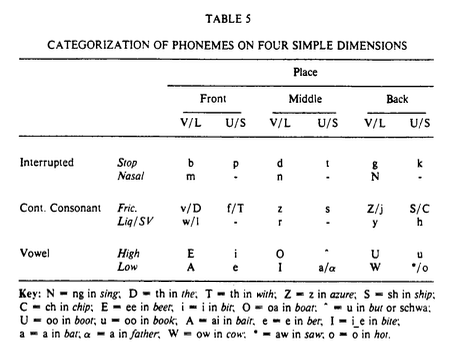
\includegraphics[scale=0.8]{img/rumelhartpreprocess.png}
    \caption{Preprocessing Table taken from \cite{rumelhart:1986} (page 235)}
    \label{fig:preprocess-rumelhart}
\end{figure}

% \chapter{Corpus}
% \label{ap:corpus}
% 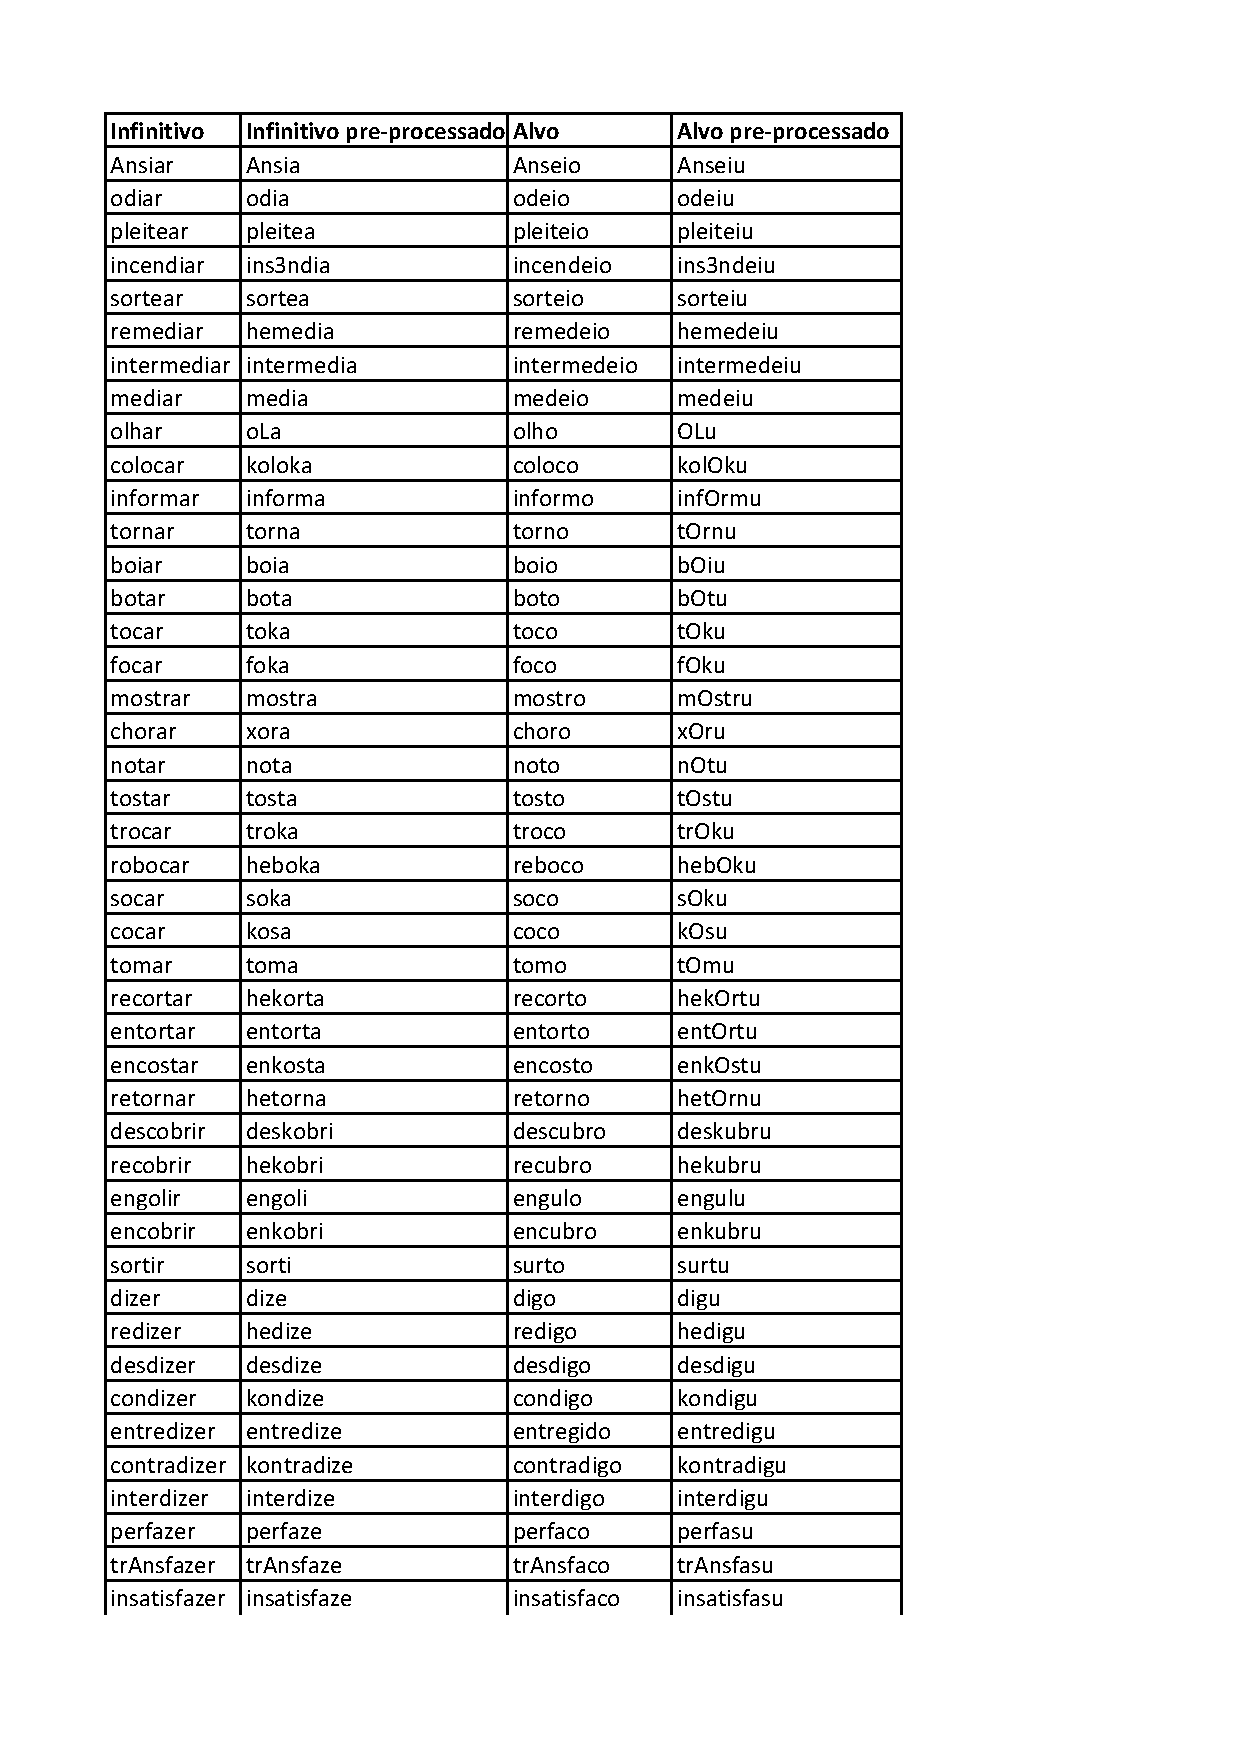
\includepdf[pagecommand={\thispagestyle{plain}},
%   pages=-]{corpus_dissertacao.pdf}

% \chapter{Resultados das Decodificações}
% \label{ap:results}
% 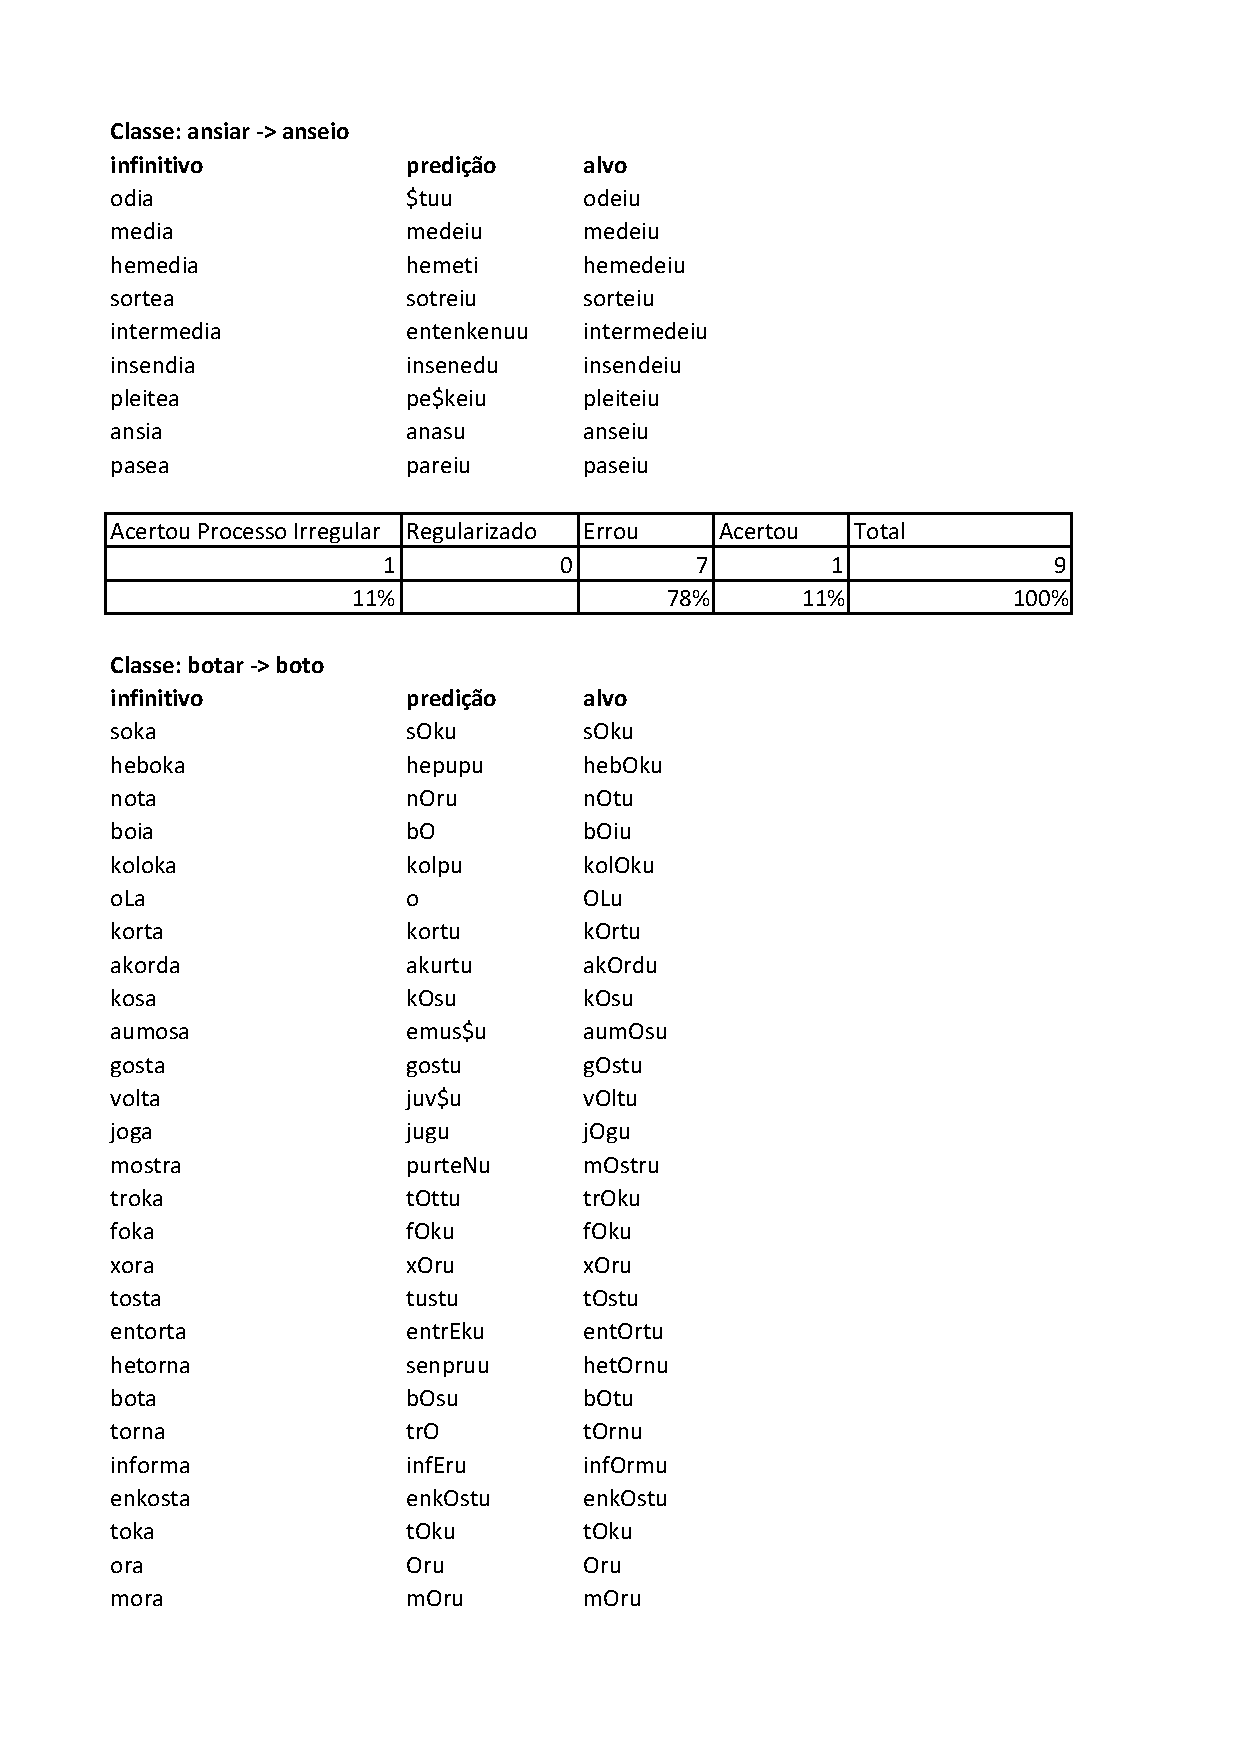
\includepdf[pagecommand={\thispagestyle{plain}},
%   pages=-]{results_analysis_by_family.pdf}

\backmatter
% cabeçalho para os apendices

% ---------------------------------------------------------------------------- %


% ---------------------------------------------------------------------------- %


% \printindex   % imprime o índice remissivo no documento 

\end{document}
